%===============================================================================
% LaTeX sjabloon voor de bachelorproef toegepaste informatica aan HOGENT
% Meer info op https://github.com/HoGentTIN/latex-hogent-report
%===============================================================================

\documentclass[dutch,dit,thesis]{hogentreport}

% TODO:
% - If necessary, replace the option `dit`' with your own department!
%   Valid entries are dbo, dbt, dgz, dit, dlo, dog, dsa, soa
% - If you write your thesis in English (remark: only possible after getting
%   explicit approval!), remove the option "dutch," or replace with "english".

\usepackage{lipsum} % For blind text, can be removed after adding actual content

\usepackage{listings}

%% Pictures to include in the text can be put in the graphics/ folder
\graphicspath{{graphics/}}

%% For source code highlighting, requires pygments to be installed
%% Compile with the -shell-escape flag!
\usepackage[section]{minted}
%% If you compile with the make_thesis.{bat,sh} script, use the following
%% import instead:
%% \usepackage[section,outputdir=../output]{minted}
\usemintedstyle{solarized-light}
\definecolor{bg}{RGB}{253,246,227} %% Set the background color of the codeframe

%% Change this line to edit the line numbering style:
\renewcommand{\theFancyVerbLine}{\ttfamily\scriptsize\arabic{FancyVerbLine}}

%% Macro definition to load external java source files with \javacode{filename}:
\newmintedfile[javacode]{java}{
    bgcolor=bg,
    fontfamily=tt,
    linenos=true,
    numberblanklines=true,
    numbersep=5pt,
    gobble=0,
    framesep=2mm,
    funcnamehighlighting=true,
    tabsize=4,
    obeytabs=false,
    breaklines=true,
    mathescape=false
    samepage=false,
    showspaces=false,
    showtabs =false,
    texcl=false,
}

\renewcommand\listoflistingscaption{%
    \IfLanguageName{dutch}{Lijst van codefragmenten}{List of listings}
}
\renewcommand\listingscaption{%
    \IfLanguageName{dutch}{Codefragment}{Listing}
}
\renewcommand*\listoflistings{%
    \addcontentsline{toc}{chapter}{\listoflistingscaption}%
    \listof{listing}{\listoflistingscaption}%
}

% Other packages not already included can be imported here


%%---------- Document metadata -------------------------------------------------
% TODO: Replace this with your own information
\author{Jamie Van Schuerbeek}
\supervisor{Mevr. C. De Leenheer}
\cosupervisor{Dhr. A. Jacobs}
\title[]%Optionele ondertitel
    {Machine learning-technologie toepassen om relevante masterdata uit bedrijfsdocumenten te halen}
\academicyear{\advance\year by -1 \the\year--\advance\year by 1 \the\year}
\examperiod{1}
\degreesought{\IfLanguageName{dutch}{Professionele bachelor in de toegepaste informatica}{Bachelor of applied computer science}}
\partialthesis{false} %% To display 'in partial fulfilment'
%\institution{Internshipcompany BVBA.}

%% Add global exceptions to the hyphenation here
\hyphenation{back-slash}
\hyphenation{tech-no-lo-gie}
\hyphenation{bed-rijfs-do-cu-men-ten}
\hyphenation{toe-pas-sen}
\hyphenation{op-ti-ma-li-se-ren}
\hyphenation{Fi-o-ri-ont-werp-richt-lij-nen}

%% The bibliography (style and settings are  found in hogentthesis.cls)
\addbibresource{bachproef.bib}            %% Bibliography file
\addbibresource{../voorstel/voorstel.bib} %% Bibliography research proposal
\defbibheading{bibempty}{}

%% Prevent empty pages for right-handed chapter starts in twoside mode
\renewcommand{\cleardoublepage}{\clearpage}

\renewcommand{\arraystretch}{1.2}

%% Content starts here.
\begin{document}

%---------- Front matter -------------------------------------------------------

\frontmatter

\hypersetup{pageanchor=false} %% Disable page numbering references
%% Render a Dutch outer title page if the main language is English
\IfLanguageName{english}{%
    %% If necessary, information can be changed here
    \degreesought{Professionele Bachelor toegepaste informatica}%
    \begin{otherlanguage}{dutch}%
       \maketitle%
    \end{otherlanguage}%
}{}

%% Generates title page content
\maketitle
\hypersetup{pageanchor=true}

%%=============================================================================
%% Voorwoord
%%=============================================================================

\chapter*{\IfLanguageName{dutch}{Woord vooraf}{Preface}}%
\label{ch:voorwoord}

%% TODO:
%% Het voorwoord is het enige deel van de bachelorproef waar je vanuit je
%% eigen standpunt (``ik-vorm'') mag schrijven. Je kan hier bv. motiveren
%% waarom jij het onderwerp wil bespreken.
%% Vergeet ook niet te bedanken wie je geholpen/gesteund/... heeft

Met veel trots presenteer ik u mijn bachelorproef, die het sluitstuk van mijn opleiding vormt en het resultaat is van lang onderzoek in een onderwerp waar ik daarvoor nog niet veel kennis over had. Machine Learning is een onderwerp dat mij erg interesseert, maar waar ik bijna geen ervaring had. Toen ik Alluvion contacteerde, met de vraag of zij een onderwerp hadden voor mijn bachelorproef, kwamen zij met het idee om een onderzoek te doen naar het gebruik van Machine Learning om bedrijfsdocumenten te analyseren. 

Ik wil daarom graag Alluvion en in het bijzonder mijn co-promotor, Alexander Jacobs, enorm bedanken voor de hulp en ondersteuning die zij mij geboden hebben voor het schrijven van deze bachelorproef. Hij heeft mij erg goed op weg kunnen helpen met het voorstellen van dit onderwerp en het geven van zeer waardevolle tips. Daarnaast wil ik ook mijn promotor, Chloé De Leenheer, bedanken voor de steun en feedback waar ik telkens op kon rekenen gedurende dit onderzoek. Tot slot wil ik ook mijn familie en vrienden bedanken voor de steun die zij mij gegeven hebben tijdens het schrijven van deze bachelorproef en gedurende mijn opleiding.
%%=============================================================================
%% Samenvatting
%%=============================================================================

% TODO: De "abstract" of samenvatting is een kernachtige (~ 1 blz. voor een
% thesis) synthese van het document.
%
% Een goede abstract biedt een kernachtig antwoord op volgende vragen:
%
% 1. Waarover gaat de bachelorproef?
% 2. Waarom heb je er over geschreven?
% 3. Hoe heb je het onderzoek uitgevoerd?
% 4. Wat waren de resultaten? Wat blijkt uit je onderzoek?
% 5. Wat betekenen je resultaten? Wat is de relevantie voor het werkveld?
%
% Daarom bestaat een abstract uit volgende componenten:
%
% - inleiding + kaderen thema
% - probleemstelling
% - (centrale) onderzoeksvraag
% - onderzoeksdoelstelling
% - methodologie
% - resultaten (beperk tot de belangrijkste, relevant voor de onderzoeksvraag)
% - conclusies, aanbevelingen, beperkingen
%
% LET OP! Een samenvatting is GEEN voorwoord!

%%---------- Nederlandse samenvatting -----------------------------------------
%
% TODO: Als je je bachelorproef in het Engels schrijft, moet je eerst een
% Nederlandse samenvatting invoegen. Haal daarvoor onderstaande code uit
% commentaar.
% Wie zijn bachelorproef in het Nederlands schrijft, kan dit negeren, de inhoud
% wordt niet in het document ingevoegd.

\IfLanguageName{english}{%
\selectlanguage{dutch}
\chapter*{Samenvatting}
\lipsum[1-4]
\selectlanguage{english}
}{}

%%---------- Samenvatting -----------------------------------------------------
% De samenvatting in de hoofdtaal van het document

\chapter*{\IfLanguageName{dutch}{Samenvatting}{Abstract}}
Alluvion is een bedrijf dat software as a service- (SaaS) en eigen SAP softwareoplossingen biedt alsook consulting met betrekking tot SAP master data kwaliteit en bedrijfsprocess optimalisatie.

In het dynamische landschap van de moderne bedrijfsvoering, is het efficiënt master data uit omvangrijke bedrijfsdocumenten halen cruciaal. In de meeste bedrijven wordt dit nog steeds beschouwd als een overbodige handmatige activiteit. Masterdata, de kerninformatie die de belangrijkste entiteiten van een organisatie definieert zoals klanten, producten en leveranciers, speelt een belangrijke rol bij geïnformeerde besluitvorming en strategische planning. Hoe kan machine learning-technologie worden toegepast om relevante masterdata uit bedrijfsdocumenten te halen? Met dit onderzoek zou Alluvion graag een antwoord op deze vraag willen krijgen door de verschillende manieren om dit proces te automatiseren te ontdekken.

Om dit doel te bereiken begint deze studie met een onderzoek naar deep learning technieken zoals, Natural Language Processing (NLP) en Information Extraction (IE), die kunnen gebruikt worden om dit doel te bereiken. Vervolgens wordt er ook onderzoek gedaan naar bestaande tools die deze technieken implementeren, zoals SAP Business Entity Recognition (BER). Deze tools worden vervolgens geëvalueerd op basis van verschillende factoren zoals prijs, kwaliteit, integratie met SAP platformen en gebruiksvriendelijkheid om zo een tool te kunnen bepalen waarmee een proof of concept wordt gemaakt.

Een praktische implementatie in de vorm van een proof of concept toont aan hoe de SAP BER service gebruikt kan worden om een praktische toepassing te maken die masterdata uit bedrijfsdocumenten kan halen. Dit proof of concept dient als een basis voor verdere ontwikkeling van een product dat Alluvion kan gebruiken om verdere verbeteringen aan te maken om op die manier een volledig product te bekomen. SAP BER samen gepaard met SAP Fiori vormt een eenvoudige manier om applicaties te bouwen die kunnen helpen bij het automatiseren van masterdata extractie uit bedrijfsdocumenten.



%---------- Inhoud, lijst figuren, ... -----------------------------------------

\tableofcontents

% In a list of figures, the complete caption will be included. To prevent this,
% ALWAYS add a short description in the caption!
%
%  \caption[short description]{elaborate description}
%
% If you do, only the short description will be used in the list of figures

\listoffigures

% If you included tables and/or source code listings, uncomment the appropriate
% lines.
\listoftables
\listoflistings

% Als je een lijst van afkortingen of termen wil toevoegen, dan hoort die
% hier thuis. Gebruik bijvoorbeeld de ``glossaries'' package.
% https://www.overleaf.com/learn/latex/Glossaries

%---------- Kern ---------------------------------------------------------------

\mainmatter{}

% De eerste hoofdstukken van een bachelorproef zijn meestal een inleiding op
% het onderwerp, literatuurstudie en verantwoording methodologie.
% Aarzel niet om een meer beschrijvende titel aan deze hoofdstukken te geven of
% om bijvoorbeeld de inleiding en/of stand van zaken over meerdere hoofdstukken
% te verspreiden!

%%=============================================================================
%% Inleiding
%%=============================================================================

\chapter{\IfLanguageName{dutch}{Inleiding}{Introduction}}%
\label{ch:inleiding}

%De inleiding moet de lezer net genoeg informatie verschaffen om het onderwerp te begrijpen en in te zien waarom de onderzoeksvraag de moeite waard is om te onderzoeken. In de inleiding ga je literatuurverwijzingen beperken, zodat de tekst vlot leesbaar blijft. Je kan de inleiding verder onderverdelen in secties als dit de tekst verduidelijkt. Zaken die aan bod kunnen komen in de inleiding~\autocite{Pollefliet2011}:

% \begin{itemize}
%   \item context, achtergrond
%   \item afbakenen van het onderwerp
%   \item verantwoording van het onderwerp, methodologie
%   \item probleemstelling
%   \item onderzoeksdoelstelling
%   \item onderzoeksvraag
%   \item \ldots
% \end{itemize}

In deze tijd is data niet meer weg te denken en is het een van de belangrijkste zaken in de bedrijfswereld, een bedrijf dat dan ook efficiënt omgaat met zijn master data kan op die manier meer geïnformeerde beslissingen maken. Omdat het ophalen van interessante data uit bedrijfsdocumenten voor veel bedrijven nog een manuele taak blijft, is een oplossing die meer geautomatiseerd is steeds interessanter aan het worden. De bedoeling van dit onderzoek is manieren te vinden om relevante informatie uit bedrijfsdocumenten te halen, nadien een werkend prototype te maken voor deze oplossing en dit te integreren in het SAP Master Data Governance platform om op deze manier master data records aan te maken. Op deze manier kan met behulp van machine learning de anderzijds manuele taak van informatie extractie geautomatiseerd worden.

\section{\IfLanguageName{dutch}{Probleemstelling}{Problem Statement}}%
\label{sec:probleemstelling}

Het gebruik van machine learning-technologie wordt tegenwoordig steeds meer toegepast. Maar hoe kan deze technologie worden gebruikt om relevante masterdata uit bedrijfsdocumenten te halen? Alluvion, een bedrijf gespecialiseerd in het gebruik van SAP Master Data management, wil graag weten hoe deze technologie gebruikt kan worden om deze, vaak nog manuele, taak te automatiseren. Door onderzoek te doen naar bestaande technologieën en tools en het maken van een proof of concept, kan Alluvion een beter beeld krijgen in de mogelijkheden en werking van deze technologieën.
\section{\IfLanguageName{dutch}{Onderzoeksvraag}{Research question}}%
\label{sec:onderzoeksvraag}
% Wees zo concreet mogelijk bij het formuleren van je onderzoeksvraag. Een onderzoeksvraag is trouwens iets waar nog niemand op dit moment een antwoord heeft (voor zover je kan nagaan). Het opzoeken van bestaande informatie (bv. ``welke tools bestaan er voor deze toepassing?'') is dus geen onderzoeksvraag. Je kan de onderzoeksvraag verder specifiëren in deelvragen. Bv.~als je onderzoek gaat over performantiemetingen, dan 
Dit onderzoek bevat een hoofd onderzoeksvraag:
Hoe kan machine learning-technologie worden toegepast om relevante masterdata uit bedrijfsdocumenten te halen?

Verder zijn er nog een deelvraag:

Welke tools bestaan er die gebruikt kunnen worden een dergelijke oplossing te maken?

\section{\IfLanguageName{dutch}{Onderzoeksdoelstelling}{Research objective}}%
\label{sec:onderzoeksdoelstelling}

%Wat is het beoogde resultaat van je bachelorproef? Wat zijn de criteria voor succes? Beschrijf die zo concreet mogelijk. Gaat het bv.\ om een proof-of-concept, een prototype, een verslag met aanbevelingen, een vergelijkende studie, enz.
De doelstelling van dit onderzoek is door een literatuurstudie een inzicht te krijgen over de verschillende onderwerpen die relevant zijn in dit onderzoek. Vervolgens is het de bedoeling om een proof of concept te maken die aantoont hoe de kennis uit de literatuuurstudie kan worden toegepast om een applicatie te maken die dient als basis voor een dienst die verder uitgebreid kan worden.  

\section{\IfLanguageName{dutch}{Opzet van deze bachelorproef}{Structure of this bachelor thesis}}%
\label{sec:opzet-bachelorproef}

% Het is gebruikelijk aan het einde van de inleiding een overzicht te
% geven van de opbouw van de rest van de tekst. Deze sectie bevat al een aanzet
% die je kan aanvullen/aanpassen in functie van je eigen tekst.

De rest van deze bachelorproef is als volgt opgebouwd:

In Hoofdstuk~\ref{ch:stand-van-zaken} wordt een overzicht gegeven van de stand van zaken binnen het onderzoeksdomein, op basis van een literatuurstudie.

In Hoofdstuk~\ref{ch:methodologie} wordt de methodologie toegelicht en worden de gebruikte onderzoekstechnieken besproken om een antwoord te kunnen formuleren op de onderzoeksvragen.

% TODO: Vul hier aan voor je eigen hoofstukken, één of twee zinnen per hoofdstuk
In Hoofdstuk~\ref{ch:proof-of-concept} wordt de toepassing toegelicht die een oplossing op de probleemstelling biedt.

In Hoofdstuk~\ref{ch:conclusie}, tenslotte, wordt de conclusie gegeven en een antwoord geformuleerd op de onderzoeksvragen. Daarbij wordt ook een aanzet gegeven voor toekomstig onderzoek binnen dit domein.
\chapter{\IfLanguageName{dutch}{Stand van zaken}{State of the art}}%
\label{ch:stand-van-zaken}

% Tip: Begin elk hoofdstuk met een paragraaf inleiding die beschrijft hoe
% dit hoofdstuk past binnen het geheel van de bachelorproef. Geef in het
% bijzonder aan wat de link is met het vorige en volgende hoofdstuk.

% Pas na deze inleidende paragraaf komt de eerste sectiehoofding.

%Dit hoofdstuk bevat je literatuurstudie. De inhoud gaat verder op de inleiding, maar zal het onderwerp van de bachelorproef *diepgaand* uitspitten. De bedoeling is dat de lezer na lezing van dit hoofdstuk helemaal op de hoogte is van de huidige stand van zaken (state-of-the-art) in het onderzoeksdomein. Iemand die niet vertrouwd is met het onderwerp, weet nu voldoende om de rest van het verhaal te kunnen volgen, zonder dat die er nog andere informatie moet over opzoeken \autocite{Pollefliet2011}.

%Je verwijst bij elke bewering die je doet, vakterm die je introduceert, enz.\ naar je bronnen. In \LaTeX{} kan dat met het commando \texttt{$\backslash${textcite\{\}}} of \texttt{$\backslash${autocite\{\}}}. Als argument van het commando geef je de ``sleutel'' van een ``record'' in een bibliografische databank in het Bib\LaTeX{}-formaat (een tekstbestand). Als je expliciet naar de auteur verwijst in de zin (narratieve referentie), gebruik je \texttt{$\backslash${}textcite\{\}}. Soms is de auteursnaam niet expliciet een onderdeel van de zin, dan gebruik je \texttt{$\backslash${}autocite\{\}} (referentie tussen haakjes). Dit gebruik je bv.~bij een citaat, of om in het bijschrift van een overgenomen afbeelding, broncode, tabel, enz. te verwijzen naar de bron. In de volgende paragraaf een voorbeeld van elk.

%\textcite{Knuth1998} schreef een van de standaardwerken over sorteer- en zoekalgoritmen. Experten zijn het erover eens dat cloud computing een interessante opportuniteit vormen, zowel voor gebruikers als voor dienstverleners op vlak van informatietechnologie~\autocite{Creeger2009}.

%Let er ook op: het \texttt{cite}-commando voor de punt, dus binnen de zin. Je verwijst meteen naar een bron in de eerste zin die erop gebaseerd is, dus niet pas op het einde van een paragraaf.

%\lipsum[7-20]

In de stand van zaken wordt er informatie gegeven over de verschillende onderwerpen omtrent de extractie van informatie uit documenten met behulp van artificiële intelligentie. Allereest wordt er toegelicht wat information extraction precies inhoudt. Daarna wordt er uitleg gegeven over Named Entity Recognition, wat een onderdeel is van Information Extraction. Verder wordt er uitgelegd hoe dit gerealiseerd kan worden aan de hand van artificiële intelligentie en deep learning. Tot slot is er nog uitleg over verschillende soorten libraries, die vaak een grote rol spelen in het ontwikkelen van zulke toepassingen.

\section{Master data en master data management}

\textcite{loshin2010master} definieert master data als belangrijke bedrijfsobjecten die gebruikt worden in verschillende applicaties binnen de organisatie, zoals klanten, leveranciers, werknemers, producten \ldots. Master data bestaat doorgaands in meer dan één bepaald deel van het bedrijf, zo kan een klant bijvoorbeeld zowel in de boekhouding als in de verkoopafdeling voorkomen. Naast dat master data cruciaal is voor de werking van de systemen binnen een bedrijf, kunnen de catergorieën van master data ook gebruikt worden om raporten en inzichten te maken zoals bijvoorbeeld: verkopen per klant per regio \autocite{loshin2010master}.

Master data management omvat het ontwikkelen van één bron van waarheid voor de master data van een bedrijf. Om dit te bereiken wordt de data gede-dupliceerd, afgestemd op elkaar en verrijkt om een consistente en betrouwbare bron te worden \autocite{silvola2011managing}. 

Een doeleinde waar master data management wordt toegepast is Enterprise Resource Plannning (ERP). ERP volgt een aanpak waarbij Bedrijfsprocessen centraal staan en intergreert master data langs deze processen. Dit zorgt ervoor dat alle processen, maar vooral de master data centraal wordt beheerd en dat dit consistent blijft \autocite{maedche2010erp}.

\section{SAP}

SAP is een van de grootste ontwikkelaars van bedrijfsmanagement-software. SAP is opgestart in 1972 door 5 personen en nu een grote multinational met meer dan 105.000 werknemers. SAP is begonnen met het maken van Enterprise Resource Planning (ERP) software, met als voriges versies: SAP R/2 en SAP R/3 en neemt ERP naar een nieuw niveau door SAP S/4HANA. In deze versie gebruiken ze nieuwe in-memory technologieën om grote aantallen data te kunnen verwerken, ook gebruiken ze nieuwe zaken zoals: cloud, AI en machine learning om de workflow van klanten verder te versnellen \autocite{SAP} 

\section{Enterprise Resource Planning}

Enterprise Resource Planning (ERP) is volgens \textcite{SAPERP} een softwaresysteem dat bedrijven helpt om hun zaak te draaien en processen te ondersteunen. In het kort helpt een ERP systeem om efficiënt grote processen zoals: Boekhouding, HR, productie\ldots. samen te brengen en te ondersteunen. Dit zorgt ervoor dat alle data centraal via 1 systeem wordt beheerd en alles simpel doorgegeven kan worden tussen de verschillende diensten. \textcite{SAPERP} geeft dan ook aan dat de moderne ERP-systemen alles behalve een simpel stukje software zijn, maar tegenwoordig via de cloud en met de nieuwste technologieën worden geleverd.

\begin{figure}[h]
  \centering
  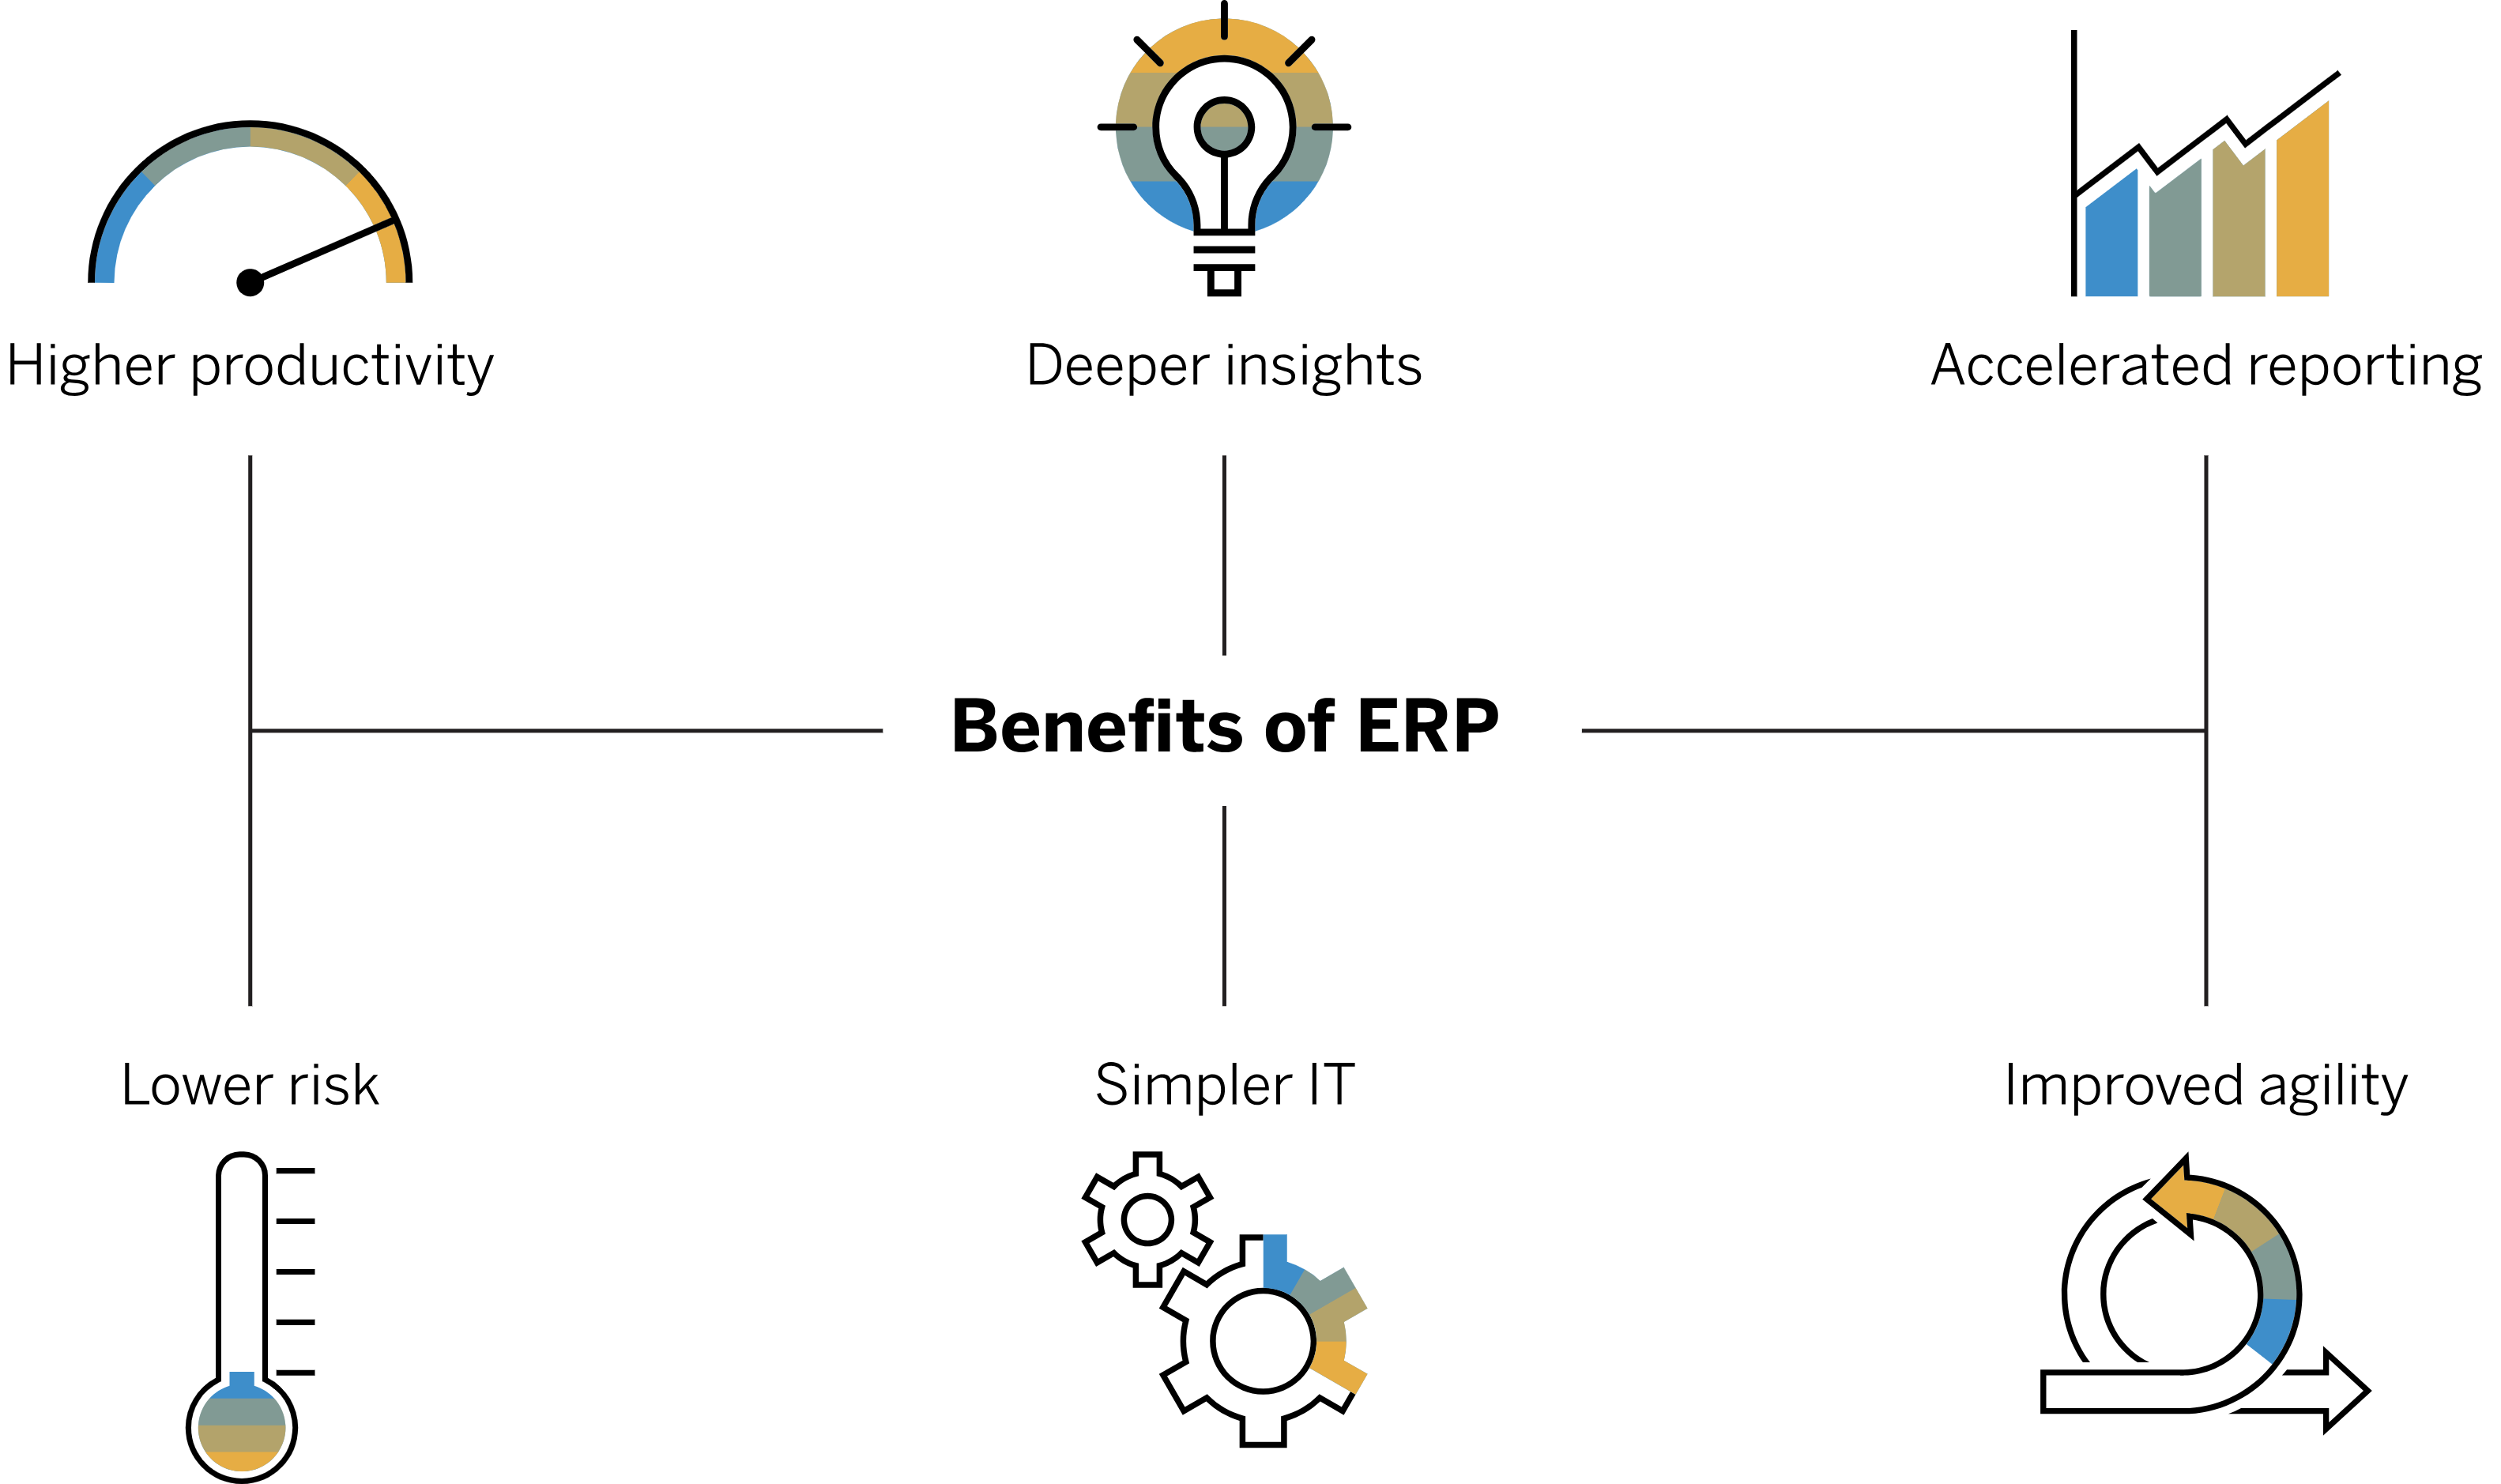
\includegraphics[width=.8\textwidth]{./graphics/erp-benefits}
  \caption{\label{fig:benefitserp}Voordelen van een ERP-systeem \autocite{SAPERP}}
\end{figure}

Volgens \textcite{SAPERP} zijn er dan ook verschillende voordelen aan het gebruiken van een ERP-systeem:
\begin{itemize}
  \item \textbf{Hogere productiviteit:} Bedrijfsprocessen automatiseren en optimaliseren om iedereen meer te laten doen met minder middelen.
  \item \textbf{Beter inzicht:} Een enkele opslag van data, een bron van data die antwoord kan geven op alle bedrijfsvragen.
  \item \textbf{Snellere rapportage:} Versnelde rapportage en gemakkelijk resultaten delen. Sneller actie nemen en prestatie verbeteren.
  \item \textbf{Minder risico:} Verzeker dat het bedrijf regelementair in orde is en risico velagen.
  \item \textbf{Simplere IT:} Geef IT een gemakkelijkere manier om te werken door alles te integreren in een ERP-systeem.
  \item \textbf{Meer flexibiliteit:} Met efficiënte operaties en directe toegang tot realtime gegevens kan er sneller nieuwe kansen identificeren en erop reageren.
\end{itemize}
\section{Information Extraction}

Information Extraction(IE) is een manier om tekst te doorzoeken met als doel belanghebbende informatie te vinden voor bepaalde doeleinden. Het omvangt meer dan enkel en alleen trefwoorden te zoeken in de tekst, maar de doelstellingen blijven achter bij het probleem van tekstbegrip, waarbij we proberen alle informatie in een tekst vast te leggen, samen met de intentie van de schrijver \autocite{hobbs2010}. Volgens \textcite{Freitag2000} is IE het probleem van het samenvatten van essentiële details die specefiek zijn voor een bepaald documenten. Een apparte samenvatting gemaakt door een computerprogramma zal een template aanhouden die bepaalde velden invult aan de hand van de tekst uit het document.

IE ligt tussen twee andere methodes van tekstverwerking, namelijk information retrieval en natuurlijke taalverwerking. IE kan worden beschouwd als een soort goedkoop, gericht begrijpen van natuurlijke taal. IE gaat uit van een verzameling documenten, waarin elk document namen en gebeurtenissen beschrijft die op elkaar lijken, maar waar de details verschillen. Voor een IE-taak wordt er een sjabloon voorzien die beschrijft wat voor informatie er in het document staat \autocite{Freitag2000}

\section{Natural language processing}

\textcite{allen2003natural} zegt dat natural language processing(NLP) verwijst naar computersystemen die menselijke talen, zoals Engels, Italiaans of Russisch, analyseren, proberen te begrijpen of produceren. Hij zegt dat doordat natuurlijke taal niet altijd een vaste structuur heeft, dat dit een hele complex probleem is en dat het ook meeste technieken om programmeertalen te begrijpen onbruikbaar maken. Volgens \textcite{Nadkarni2011} zijn er verschillende fases die er bij NLP worden uitgevoerd om een tekst te kunnen begrijpen. Dit begint met het afbakenen van zinnen, wat moeilijker wordt gemaakt door zaken als afkortingen en titels die ook met een punt worden afgesloten. De verdere fases zijn: identificeren van individuele woorden, categoriseren van deze woorden zoals: werkwoorden, ontleden van samenstellingen, delen van een zin markeren die bij elkaar horen zoals: bijvoeglijke naamwoorden voor een zelfstandig naamwoord en tot slot het opdelen in verschillende groepen.

\section{Named Entity Recognition}

Volgens \textcite{Mansouri2008} is Named Entity Recognition(NER) een onderdeel van Information Extraction, het omvat het verwerken van text om zo uitdrukkingen te identificeren die naar mensen, plaatsen, organisaties... verwijzen. Zij verwijzen naar twee taken die bij NER worden gedaan, als eerste worden de eniteiten uit een tekst herkend, daarna worden deze eniteiten opgedeeld in een categorie waar ze toebehoren. NER is een kritiek onderdeel in Natural language processing(NLP) wat gebruikt wordt in onder andere voice assistants zoals Siri en Alexa dit om zaken uit een gesprek te herkenen zoals plaatsen, namen... en hier een gepast antwoord op te kunnen geven. \autocite{Monaikul_2021}

\section{Artificiële intelligentie en Deep Learning}

Om een IE toepassing te maken wordt er tegenwoordig gebruik gemaakt van artificiële intelligentie(AI) of een vorm van deep learning(DL) \autocite{Yang2022}. Deep learning is een onderdeel van machine learning wat beter presteerd op ongestructureerde data. Dit omdat de algoritsmes gegevens door verschillende lagen laat die kenmerken opmerkt en doorgeeft aan de volgende, die de kenmerken samen zetten om een volledige representatie te hebben. \autocite{mathew2021deep}. \textcite{roberts2022principles} geeft aan dat deep learning artificiële neurale netwerken gebruikt en dat het lichtelijk gebaseerd is op echte biologisch neurale netwerken zoals het brein. Wel geeft \textcite{roberts2022principles} aan dat deze artificiële neurale netwerken meer moeten gezien worden als een stel functies gebouwd uit een stel rekenblokken genaamd 'neurons'.

Binnen IE ondergaat de tekst eerst meerdere fases, allereerst wordt de tekst doorzocht en worden er eniteiten uitgehaald de mogelijks van belang kunnen zijn, ook wel Named Entity Recognition(NER). Hierna worden met deze eniteiten relaties gevormd, goede relaties tussen eniteiten zorgen voor een goede interpretatie van de tekst \autocite{Yang2022}. Volgens \textcite{Yang2022} is het voordeel bij het gebruik van DL bij deze toepassingen het feit dat het systeem bijleert en de resultaten die gegeven worden steeds beter worden naarmate er meer data geleverd wordt.

%\section{Natural language processing}


\section{Libraries}
\label{sec:libraries}

Om het implementeren van deze oplossingen gemakkelijker en sneller te maken zijn er verschillende libraries en diensten beschikbaar die het mogelijk maken om zulke toepassingen te bouwen.

\subsection{SAP Document information extraction}

Document information extraction(DOX) is een dienst aangeboden door SAP die het mogelijk maakt om met machine learning informatie uit documenten te halen. Op deze manier wordt het verwerken van grote hoeveelheden aan documenten die hun inhoud in titels en tabellen hebben verwerkt. Dit geeft de mogelijkheid om documenten zoals facturen en betalingsdocumenten automatisch te verwerken. In dit systeem wordt als input een document aan de API gegeven die dan een gestructureerd resultaat teruggeeft met alle verschillende velden uit het document. \autocite{SAPDOX}.

\subsection{SAP Business entity recognition}

Business entity recognition(BER) is een gelijkaardige dienst die wordt aangeboden door SAP. Het grootste verschil is dat BER het mogelijk maakt om informatie uit ongestructureerde stukken tekst te halen. Dit biedt de mogelijkheid om bijvoorbeeld de context uit e-mails te halen of het automatiseren van herhalende taken zoals het beantwoorden van vragen over de status en betaling van facturen. Hier kunnen er voorgetrainde modellen of eigen modellen gebruikt worden om ervoor te zorgen dat de resultaten geschikter zijn voor de doeleinden van de gebruiker. Deze toepassing kan helpen om het manuele en herhalende werk in een bedrijf te verminderen zodat werknemers meer tijd hebben om zich te focussen op belangrijkere zaken.

\subsection{Open source}

Op github of andere open source softwareplatformen zijn er veel verschillende libraries en tools beschikbaar die het mogelijk om dergelijke toepassingen te ontwikkelen. Deze zijn in veel verschillende programmeertalen geschreven wat het een flexibele oplossing maakt om zelf de geweste taal te kiezen. Doordat deze allemaal open source zijn, worden deze bijna allemaal gratis aangeboden aan iedereen om te gebruiken. Het grootste verschil tussen deze toepassingen en DOX of BER is het feit dat deze veelal niet automatisch een integratie hebben met een SAP systeem en dat deze zelf nog ontwikkeld moet worden.
Een paar voorbeelden van deze open source libraries zijn: 
\begin{itemize}
    \item Snips NLU - Een python library om de betekenis uit een zin te halen.
    \item MITIE - Een c++ library en tools voor information extraction.
    \item InvoiceNet - Een tool geschreven in python om informatie uit facturen te halen.
    \item \ldots
\end{itemize}

\section{SAP Fiori en SAPUI5}

SAP Fiori is een desing systeem dat het mogelijk maakt om zakelijke apps apps te maken die op elk apparaat werken. Door gebruik te maken van de Fiori-ontwerprichtilijnen en -tools kan er gemakkelijk apps gemaakt worden met een uniforme uitstraling als alle SAP-toepassingen \autocite{SAPfiori}. Fiori is ontwikkeld met het doel om een gelijke gebruikerservaring te kunnen maken voor alle SAP producten die op elk apparaat werkt. Fiori is gebouwd op SAPUI5, een library gemaakt om cross-platform webapplicaties te maken gebaseerd op HTML5 en Javascript \autocite{mathew2015beginning}.

%voorbeelden die er nog bij moeten komen: master data governance 
%%=============================================================================
%% Methodologie
%%=============================================================================

\chapter{\IfLanguageName{dutch}{Methodologie}{Methodology}}%
\label{ch:methodologie}

%% TODO: In dit hoofstuk geef je een korte toelichting over hoe je te werk bent
%% gegaan. Verdeel je onderzoek in grote fasen, en licht in elke fase toe wat
%% de doelstelling was, welke deliverables daar uit gekomen zijn, en welke
%% onderzoeksmethoden je daarbij toegepast hebt. Verantwoord waarom je
%% op deze manier te werk gegaan bent.
%% 
%% Voorbeelden van zulke fasen zijn: literatuurstudie, opstellen van een
%% requirements-analyse, opstellen long-list (bij vergelijkende studie),
%% selectie van geschikte tools (bij vergelijkende studie, "short-list"),
%% opzetten testopstelling/PoC, uitvoeren testen en verzamelen
%% van resultaten, analyse van resultaten, ...
%%
%% !!!!! LET OP !!!!!
%%
%% Het is uitdrukkelijk NIET de bedoeling dat je het grootste deel van de corpus
%% van je bachelorproef in dit hoofstuk verwerkt! Dit hoofdstuk is eerder een
%% kort overzicht van je plan van aanpak.
%%
%% Maak voor elke fase (behalve het literatuuronderzoek) een NIEUW HOOFDSTUK aan
%% en geef het een gepaste titel.

In dit hoofdstuk worden alle fasen opgelijst en uitgelegd die worden uitgevoerd in dit onderzoek. Dit begint bij de literatuurstudie en gaat verder naar de selectie van de tools. Daarna wordt de proof of concept uitgebreider uitgelegd en tot slot de reflectie op het resultaat.

\section{Literatuurstudie}

In de literatuurstudie worden de verschillende onderwerpen die relevant zijn voor het onderzoek opgelijst en verder uitgelegd. Op deze manier kan er een goede basiskennis opgebouwd worden over de verder besproken onderwerpen. Verder wordt in de literatuurstudie ook een oplijsting gemaakt van de verschillende tools die gebruikt kunnen worden om de proof of concept verder uit te bouwen. Deze lijst is geselecteerd op basis van de tools die SAP zelf aanbied en de libraries die op github aangeboden worden die de meeste sterren hebben. Aan de hand van deze resultaten kan er een keuze gemaakt worden die gebruikt worden voor de proof of concept. De keuze van deze tools kan van een aantal factoren afhangen, namelijk: benodigde programmertaal, beschikbare documentatie, eventuele beperkingen met de open source license, \ldots

\section{Selectie van geschikte tools}

Voordat er een proof of concept kan gemaakt worden moet er eerst een selectie gemaakt worden van de geschikte tools die gebruikt moeten worden. De keuze van de uiteindelijke tools wordt gedaan op basis van een aantal factoren die belangrijk zijn bij het maken van de uiteindelijke keuze.
Deze factoren zijn de volgende: 

%-	Verschillende prijzen
%-	SAP-geleverde oplossingen
%-	Kwaliteit
%-	Proces volume
%-	Mogelijke integratie met SAP platformen
%-	Connectiviteit
%-	Ease of use

\begin{itemize}
    \item Prijs van de tool
    \item Kwaliteit van het resultaat
    %\item De proces volume
    \item mogelijkheid om te integreren met SAP platformen
    \item Gebruiksvriendelijkheid
\end{itemize}

%TODO: Deze nog ff fixen. footnote werkt niet...
\begin{table}[h]
    \centering
    \tiny
    \begin{tabular}{|c|c|c|c|}
        \toprule
        factor & \textbf{SAP Business Entity Recognition}\footnote{data uit documentatie: \url{https://help.sap.com/docs/business-entity-recognition/business-entity-recognition/}} & \textbf{Snips NLU}\footnote{data uit documentatie: \url{https://snips-nlu.readthedocs.io/}} & \textbf{MITIE}\footnote{data uit de documentatie: \url{https://github.com/mit-nlp/MITIE/tree/master}} \\
        \midrule
        \textbf{Gebruiksgemak}\footnote{Minmale configuratie door de beschikbaarheid van voorgetrainde modellen} & Minimale setup, minimale configuratie & kleine setup, grote configuratie& Grote setup, mindere configuratie \\
        \textbf{SAP integratie} & Out of the box & Moet zelf gedaan worden & Moet zelf gedaan worden \\
        \textbf{Prijs} & Gratis, met limitaties & Gratis en open source & Gratis en open source \\
        \bottomrule
    \end{tabular}
    \caption{\label{tab:vergelijking}Vergelijking van tools} 
\end{table}

De gekozen tool in dit onderzoek wordt de Business Entity Recognition dienst van SAP. Dit omdat de integratie met andere tools die SAP aanbied vrij simpel kan verlopen. Door middel van een aantal api calls kan een tekst die moet worden inlezen opgestuurd worden, SAP doet verder het zware werk en geeft een resultaat terug. De grootste nadelen van deze dienst zijn het feit dat het niet gratis blijf als er een groot aantal documenten ingelezen worden en het feit dat deze niet open source is, waardoor fundamentele aanpassing aan de werking van de tool niet erg mogelijk is.
%\footnotetext{data komt uit documentatie van \href{https://help.sap.com/docs/business-entity-recognition/business-entity-recognition/}{SAP BER}, \href{https://snips-nlu.readthedocs.io/}{Snips NLU}, \href{https://github.com/mit-nlp/MITIE/tree/master/examples}{MITIE}}

\section{Proof of concept}
Om definitief een antwoord te kunnen te kunnen geven op de onderzoeksvraag uit sectie \ref{ch:inleiding}, zal er een proof of concept opgesteld worden. Deze proof of concept bestaat uit een webapplicatie die een document kan inlezen en hieruit de masterdata kan halen. Deze applicatie zal gebouwd worden doormiddel van SAP Fiori om een frontend te maken die gebruik maakt van de SAP Business Entity Recognition service om documenten op te laden en het gewenste resultaat te behalen.
\subsection{Benodigde functionaliteiten}

Tijdens het maken van de proof of concept moet er rekening gehouden worden met de verschillende functionaliteiten die de applicatie zeker moet hebben.

\begin{itemize}
    \item \textbf{Opladen van eigen gebruikersgegevens:} Om ervoor te zorgen dat een andere gebruiker de applicatie kan gebruiken met zijn eigen Business Entity Recognition instance, moet er de mogelijkheid zijn om zijn eigen configuratiebestand op te laden.
    \item \textbf{Opladen van documenten:} Om een document te laten uitlezen, moet er natuurlijk de mogelijkheid zijn om een document op te laden die gebruikt kan worden.
    \item \textbf{Eigen dataset maken:} Iedere gebruiker kan een andere interpretatie hebben over wat nu precies nuttige data is in een document. Daarom moet de applicatie de mogelijkheid hebben om een eigen dataset te maken.
    \item \textbf{dataset kiezen:} Niet elk document is hetzelfde en daarom zou er soms een andere dataset moeten kunnen gekozen worden voor een specefiek document.
\end{itemize}

\subsection{Doel}
Het doel van de proof of concept is een mogelijke oplossing maken om masterdata automatisch uit een bedrijfsdocument te halen. Deze oplossing zou in een sap systeem voor verschillende doeleinden kunnen ingezet worden om de workflow te versimpelen. Deze toepassing is bedoeld om een inkijk te kunnen geven hoe dergelijke precies gebouwd worden en hoe Alluvion zelf te werk kan gaan om een eigen applicatie te bouwen.


\section{Conclusie}
Op het einde van het onderzoek zal er een conclusie gegeven worden over de resultaten van het onderzoek en de proof of concept. Hierbij wordt er nagegaan of het onderzoek en de proof of concept de onderzoeksvraagen voldoende beantwoorden.

% Voeg hier je eigen hoofdstukken toe die de ``corpus'' van je bachelorproef
% vormen. De structuur en titels hangen af van je eigen onderzoek. Je kan bv.
% elke fase in je onderzoek in een apart hoofdstuk bespreken.

%%=============================================================================
%% Proof of concept
%%=============================================================================

\chapter{Proof of concept}%
\label{ch:proof-of-concept}

In dit hoofdstuk zal er uitgebreid besproken worden hoe de proof of concept, gebruik makend van SAP Business entity recognition, gebouwd wordt en hoe dit belanghebbende informatie uit een tekst haalt.

\section{Inhoud van de proof of concept}
De proof of concept die in dit onderzoek is gemaakt, bestaat uit een API in python die de Business Entity Recognition service van SAP aanroept en de resultaten teruggeeft. Verder bestaat de proof of concept ook uit een frontend applicatie die de API aanroept en de resultaten weergeeft. De frontend applicatie is een webapplicatie die gebruik maakt van SAP Fiori om een mooie en gebruiksvriendelijke interface te maken.
Tijdens het maken van de proof of concept is er rekening gehouden met de verschillende functionaliteiten die de applicatie zeker moet hebben. Deze functionaliteiten zijn de volgende:
\begin{itemize}
    \item Het uploaden van een service key bestand om een eigen instantie van de Business Entity Recognition service te gebruiken.
    \item Het uploaden van een tekstbestand die de service zal inlezen.
    \item Het kiezen van een bestaand model om de context van de tekst te bepalen en zo betere resultaten te verkrijgen.
    \item De mogelijkheid om de resultaten te bekijken.
\end{itemize}

\begin{figure}[H]
    \centering
    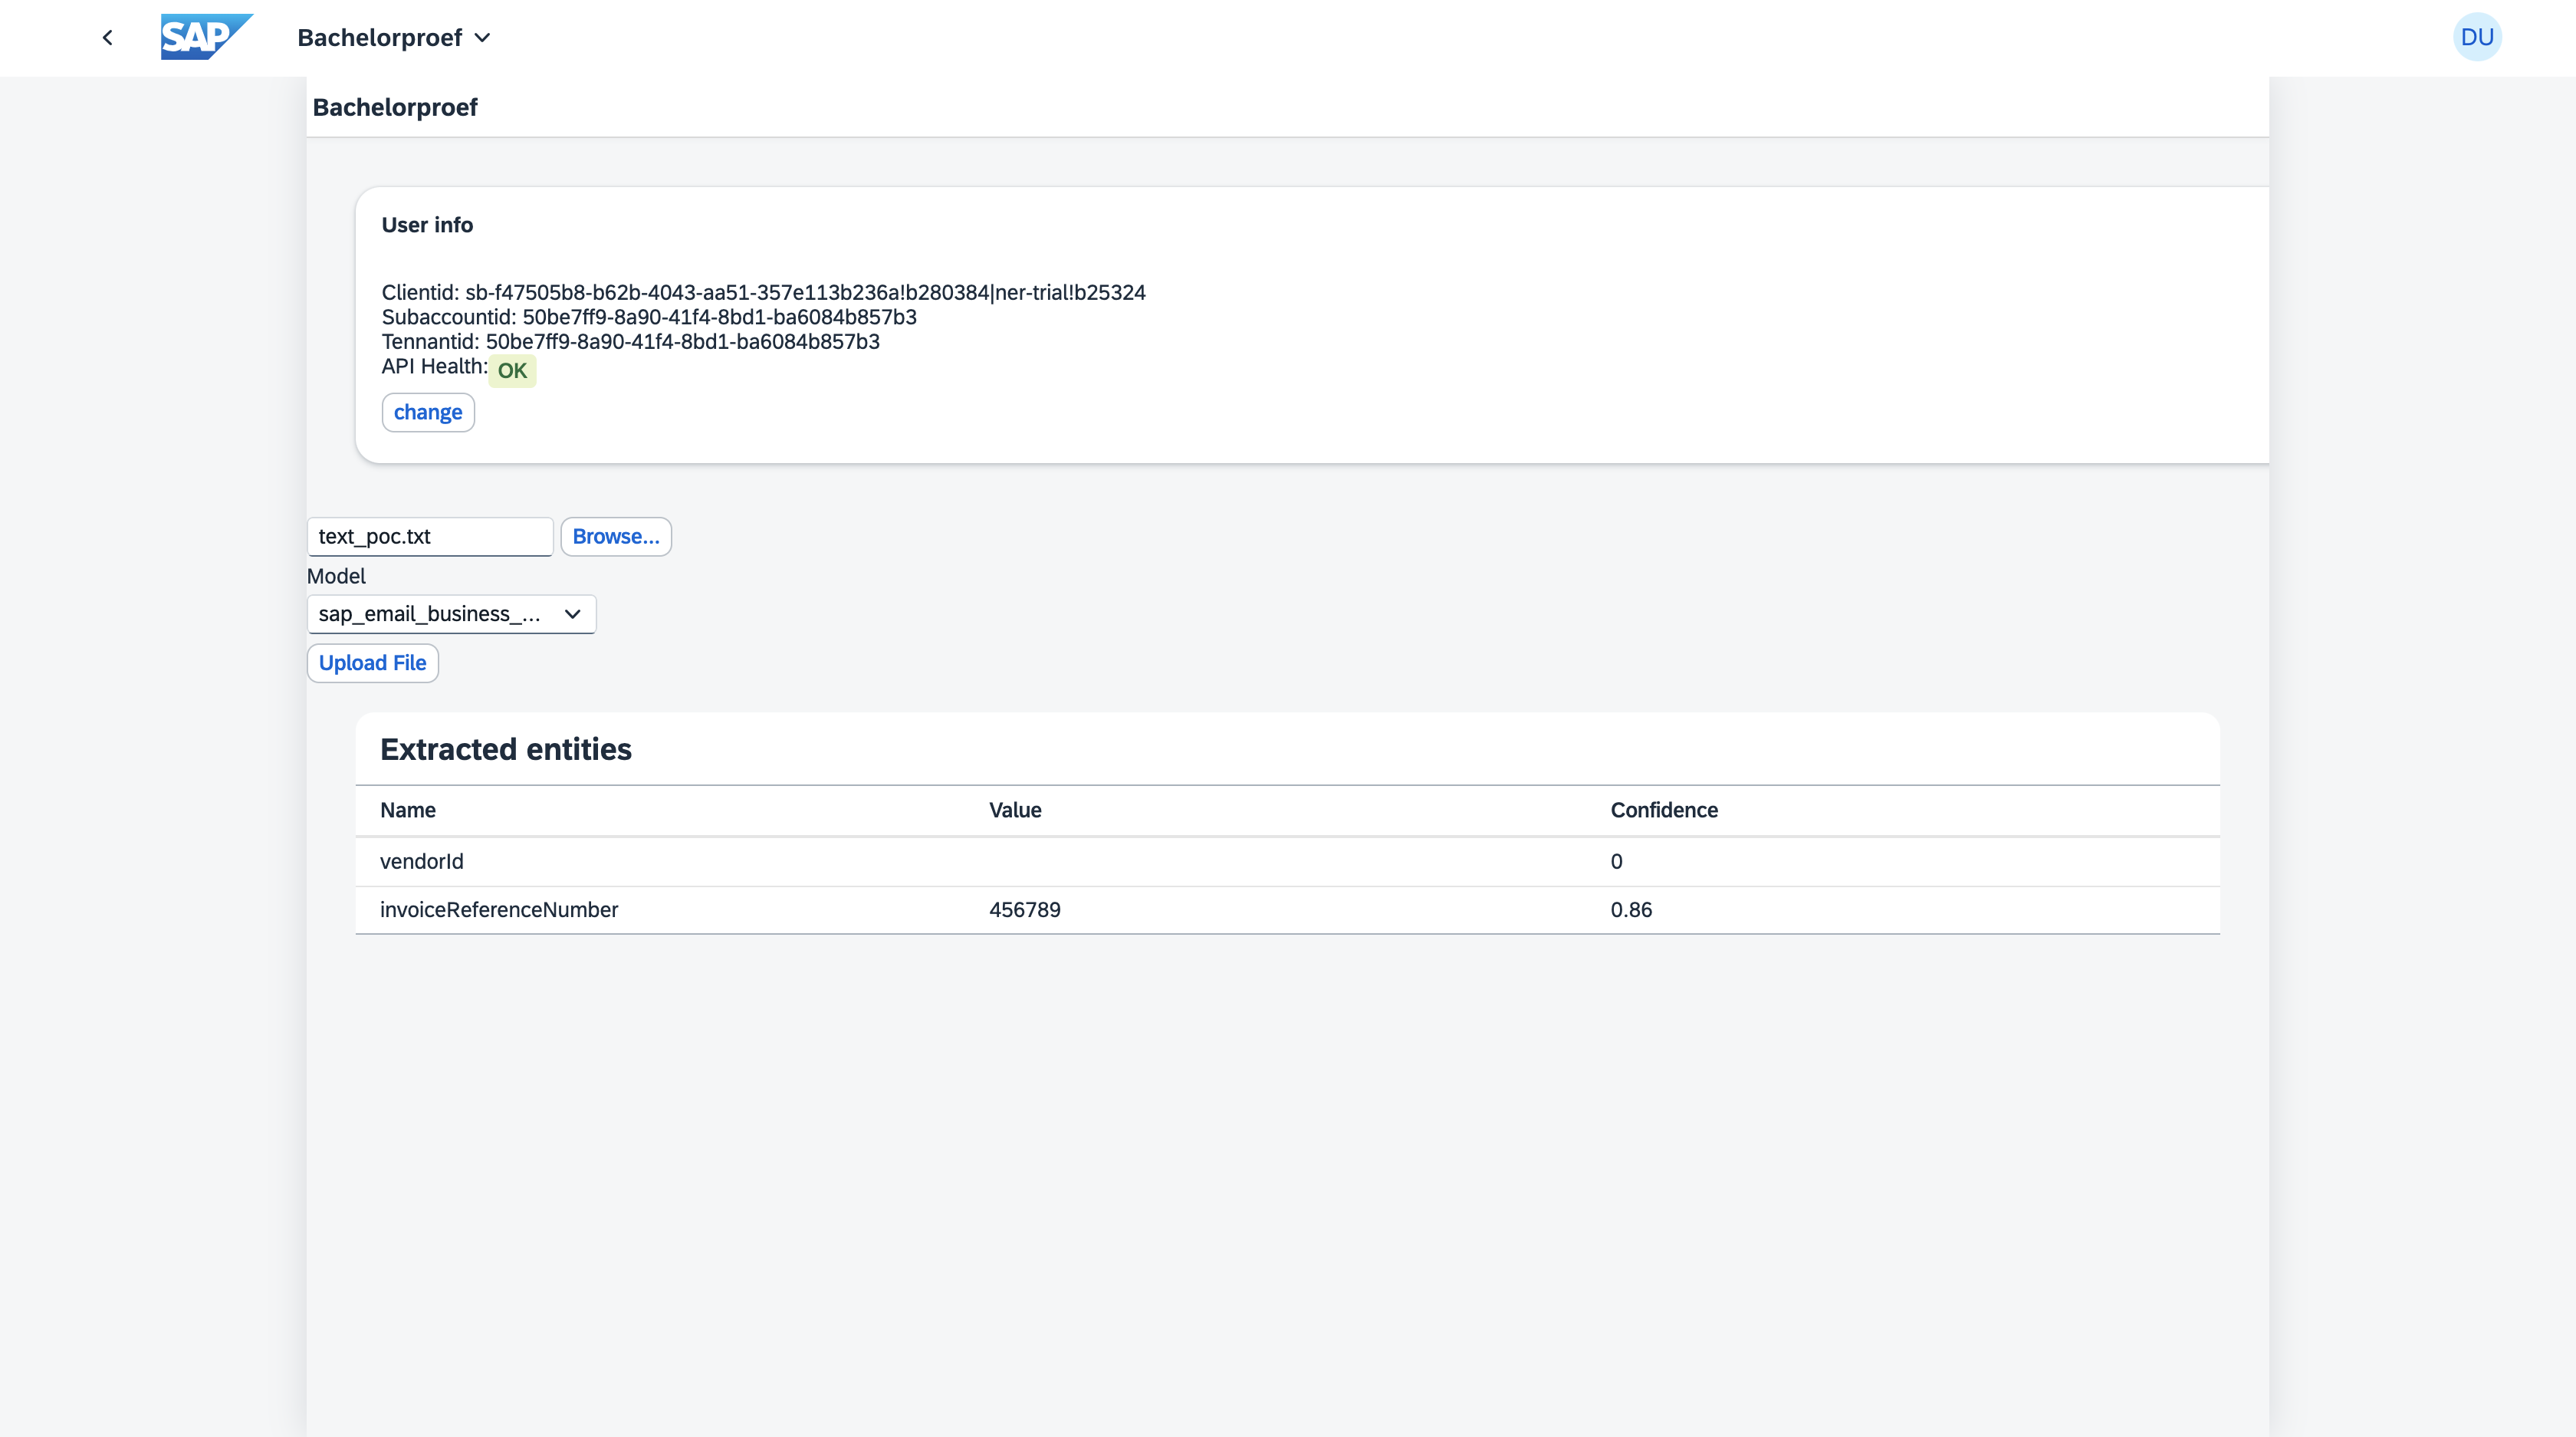
\includegraphics[width=0.8\textwidth]{./graphics/proof-of-concept.png}
    \caption{Proof of concept}
    \label{fig:proof-of-concept}
\end{figure}

\section{Benodigdheden}
Om de proof of concept uit te kunnen voeren wordt er verwacht dat er een aantal zaken reeds gekend of geïnstalleerd zijn. Deze zaken zijn de volgende:

\begin{itemize}
    \item \textbf{SAP BTP trail account:} Een trail account op de SAP Business Technology Platform (BTP) Cockpit, deze kan aangemaakt worden via: \url{https://account.hana.ondemand.com/}
    \item \textbf{Python:} Er wordt verwacht dat er een Python 3 installatie aanwezig is. Deze kan geïnstalleerd worden via: \url{https://www.python.org/downloads/}
    \item \textbf{Kennis van de gebruikte libraries:} Om de code in de proof of concept te kunnen begrijpen wordt er verwacht dat er een basiskennis van Flask en SAP Fiori aanwezig is.
    \item \textbf{Visual studio code: } Om gemakkelijk met SAP Fiori te kunnen werken wordt er aangeraden om Visual Studio Code te gebruiken. Dit omdat er een pakket met handige extensies beschikbaar is die het werken met SAP Fiori gemakkelijker maken, dit is te installeren via \url{https://marketplace.visualstudio.com/items?itemName=SAPSE.sap-ux-fiori-tools-extension-pack}. Een andere editor kan ook gebruikt worden, maar het opzetten van een project kan dan lastiger zijn.
\end{itemize}

\section{Github repository}
De volledige code van het proof-of-concept in dit onderzoek is online beschikbaar gesteld via GitHub. De repository bevat zowel de code van de api in de map \mintinline{bash}|api|, als de Fiori-applicatie in de map \mintinline{bash}|frontend|. De github repository is te vinden op \url{https://github.com/jamievschuerbeek/proof-of-concept-bachelorproef}.

\section{Opzetten van Business Entity Recognition in SAP BTP Cockpit}

Het SAP Business Technology Platform(BTP) is een online cloudplatform ontwikkeld door SAP waar er heel veel verschillende services door hen worden aangeboden en waar deze beheerd kunnen worden. De instances van deze services kunnen geheel aangepast worden aan de wensen en benodigdheden van de gebruiker doormiddel van configuratie en eigen ontwikkelingen.
Om de Business Entity Recognition service te gebruiken wordt er verwacht dat er in de SAP BTP Cockpit deze service wordt opgezet. Bij deze service kan er de configuratie aangepast worden om bijvoorbeeld eigen documenten toe te voegen die samen een dataset vormen. Deze dataset kan gebruikt worden om een eigen model te trainen.

\subsection{SAP BTP trail account}

Het SAP Business Technology Platform is opgedeeld in verschillende account: Een global account en één of meerdere subaccounts. De global account heeft toegang tot globale configuratie zoals het beheer van rollen en gebruikers die bepaalde subaccounts mogen zien en aanpassen. De subaccounts worden dan weer gebruikt om instanties van SAP-diensten op te draaien en beheren. Om op de SAP BTP Cockpit te geraken, dient er allereerst naar de homepagina van de \href{https://account.hana.ondemand.com/cockpit#/home/allaccounts}{BTP Cockpit} genavigeerd te worden. Hier kan verder via de knoppen op de pagina genavigeerd worden naar de hoofdpagina van het global trail account. Hier zijn een aantal pagina's te vinden die het mogelijk maken om verschillende zaken te beheren:
\begin{itemize}
    \item \textbf{Account explorer:} Hier kunnen de verschillende subaccounts beheerd worden.
    \item \textbf{Resource Providers:} Indien een gebruiker een eigen amazon aws of azure omgeving heeft, kan deze hier worden toegevoegd.
    \item \textbf{Boosters:} Boosters zijn tools die aangeboden worden door SAP die het gemakkelijk maken om een bepaalde service op te zetten. Meer informatie zal gegeven worden in sectie \ref{sec:ber-booster}.
    \item \textbf{System landscape:} Indien een gebruiker een SAP omgeving buiten het BTP heeft, kan deze hier worden toegevoegd.
    \item \textbf{Entitlements:} Hier kunnen de verschillende services die aangeboden worden door SAP worden beheerd.
    \item \textbf{Security:} Hier kunnen de verschillende gebruikers en rollen worden beheerd.
    \item \textbf{Usage: } Hier kan de gebruiker zien hoeveel van de verschillende services er gebruikt worden.
\end{itemize}

\subsection{Business Entity Recognition Booster}
\label{sec:ber-booster}
Om het aanmaken van de verschillende services een stuk gemakkelijker te maken, biedt SAP een aantal tools aan om deze automatisch op te zetten. Deze tools heten 'boosters' en ook voor de Business Entity Recognition service wordt er ook een booster aangeboden. Om de booster uit te voeren, dient er eerst naar de 'Boosters' pagina genavigeerd te worden op de SAP BTP Cockpit. Hier kan er gezocht worden naar de 'Set up account for Business Entity Recognition' booster en kan deze geactiveerd worden. 
\begin{figure}[H]
    \centering
    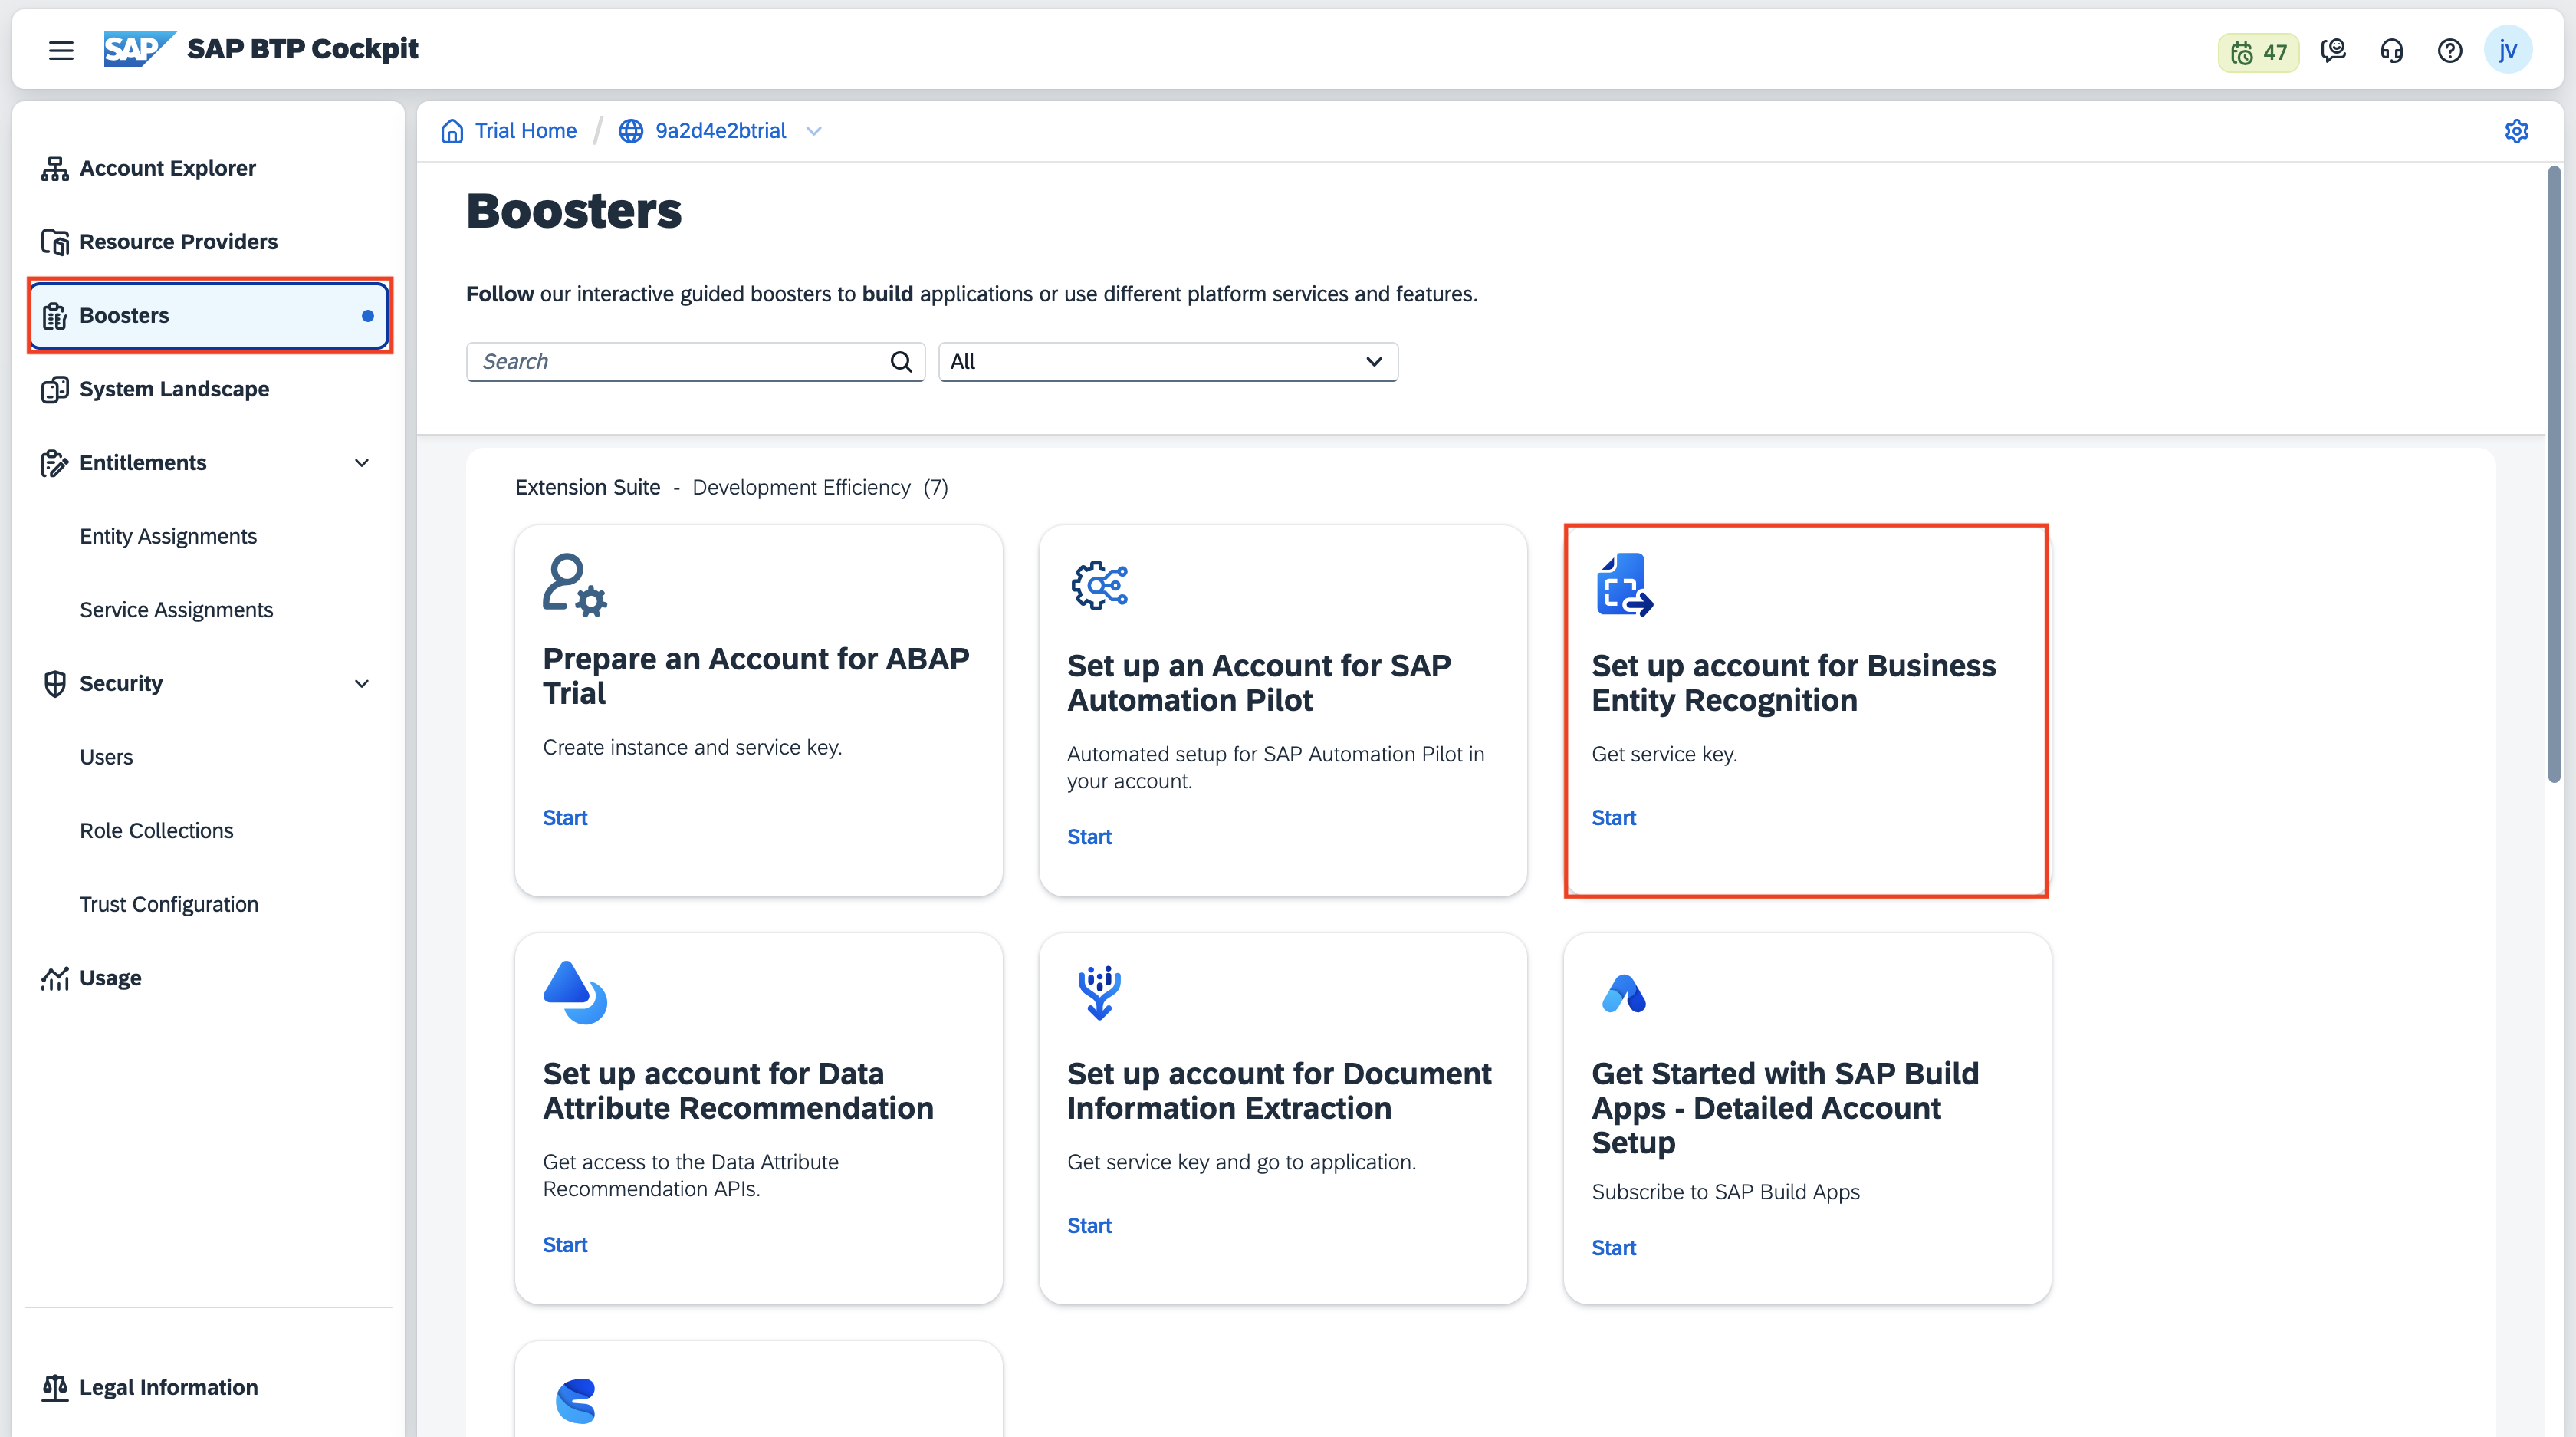
\includegraphics[width=0.8\textwidth]{./graphics/sap_btp_home_boosters.png}
    \caption{Business Entity Recognition booster}
    \label{fig:ber-booster}
\end{figure}

Na het activeren van de booster, zal er een scherm verschijnen waar de subaccount gekozen kan worden waar de service op kan draaien. Voor dit onderzoek is de standaard subaccount die aangemaakt wordt bij het aanmaken van een trail account voldoende. Verder kan er ook een space gemaakt worden waar de service in kan draaien, hiervoor is er de space 'bachelorproef' gemaakt. De booster zal dan een aantel zaken in het subaccount aanmaken en configureren, als dit allemaal gelukt is, zal er een melding verschijnen dat de booster succesvol is uitgevoerd zoals in figuur \ref{fig:booster-succes}. In deze melding staat er ook een link naar de service key die nodig is om de service aan te roepen, deze service key dient gedownload te worden en zal later in de applicatie gebruikt worden.

\begin{figure}[H]
    \centering
    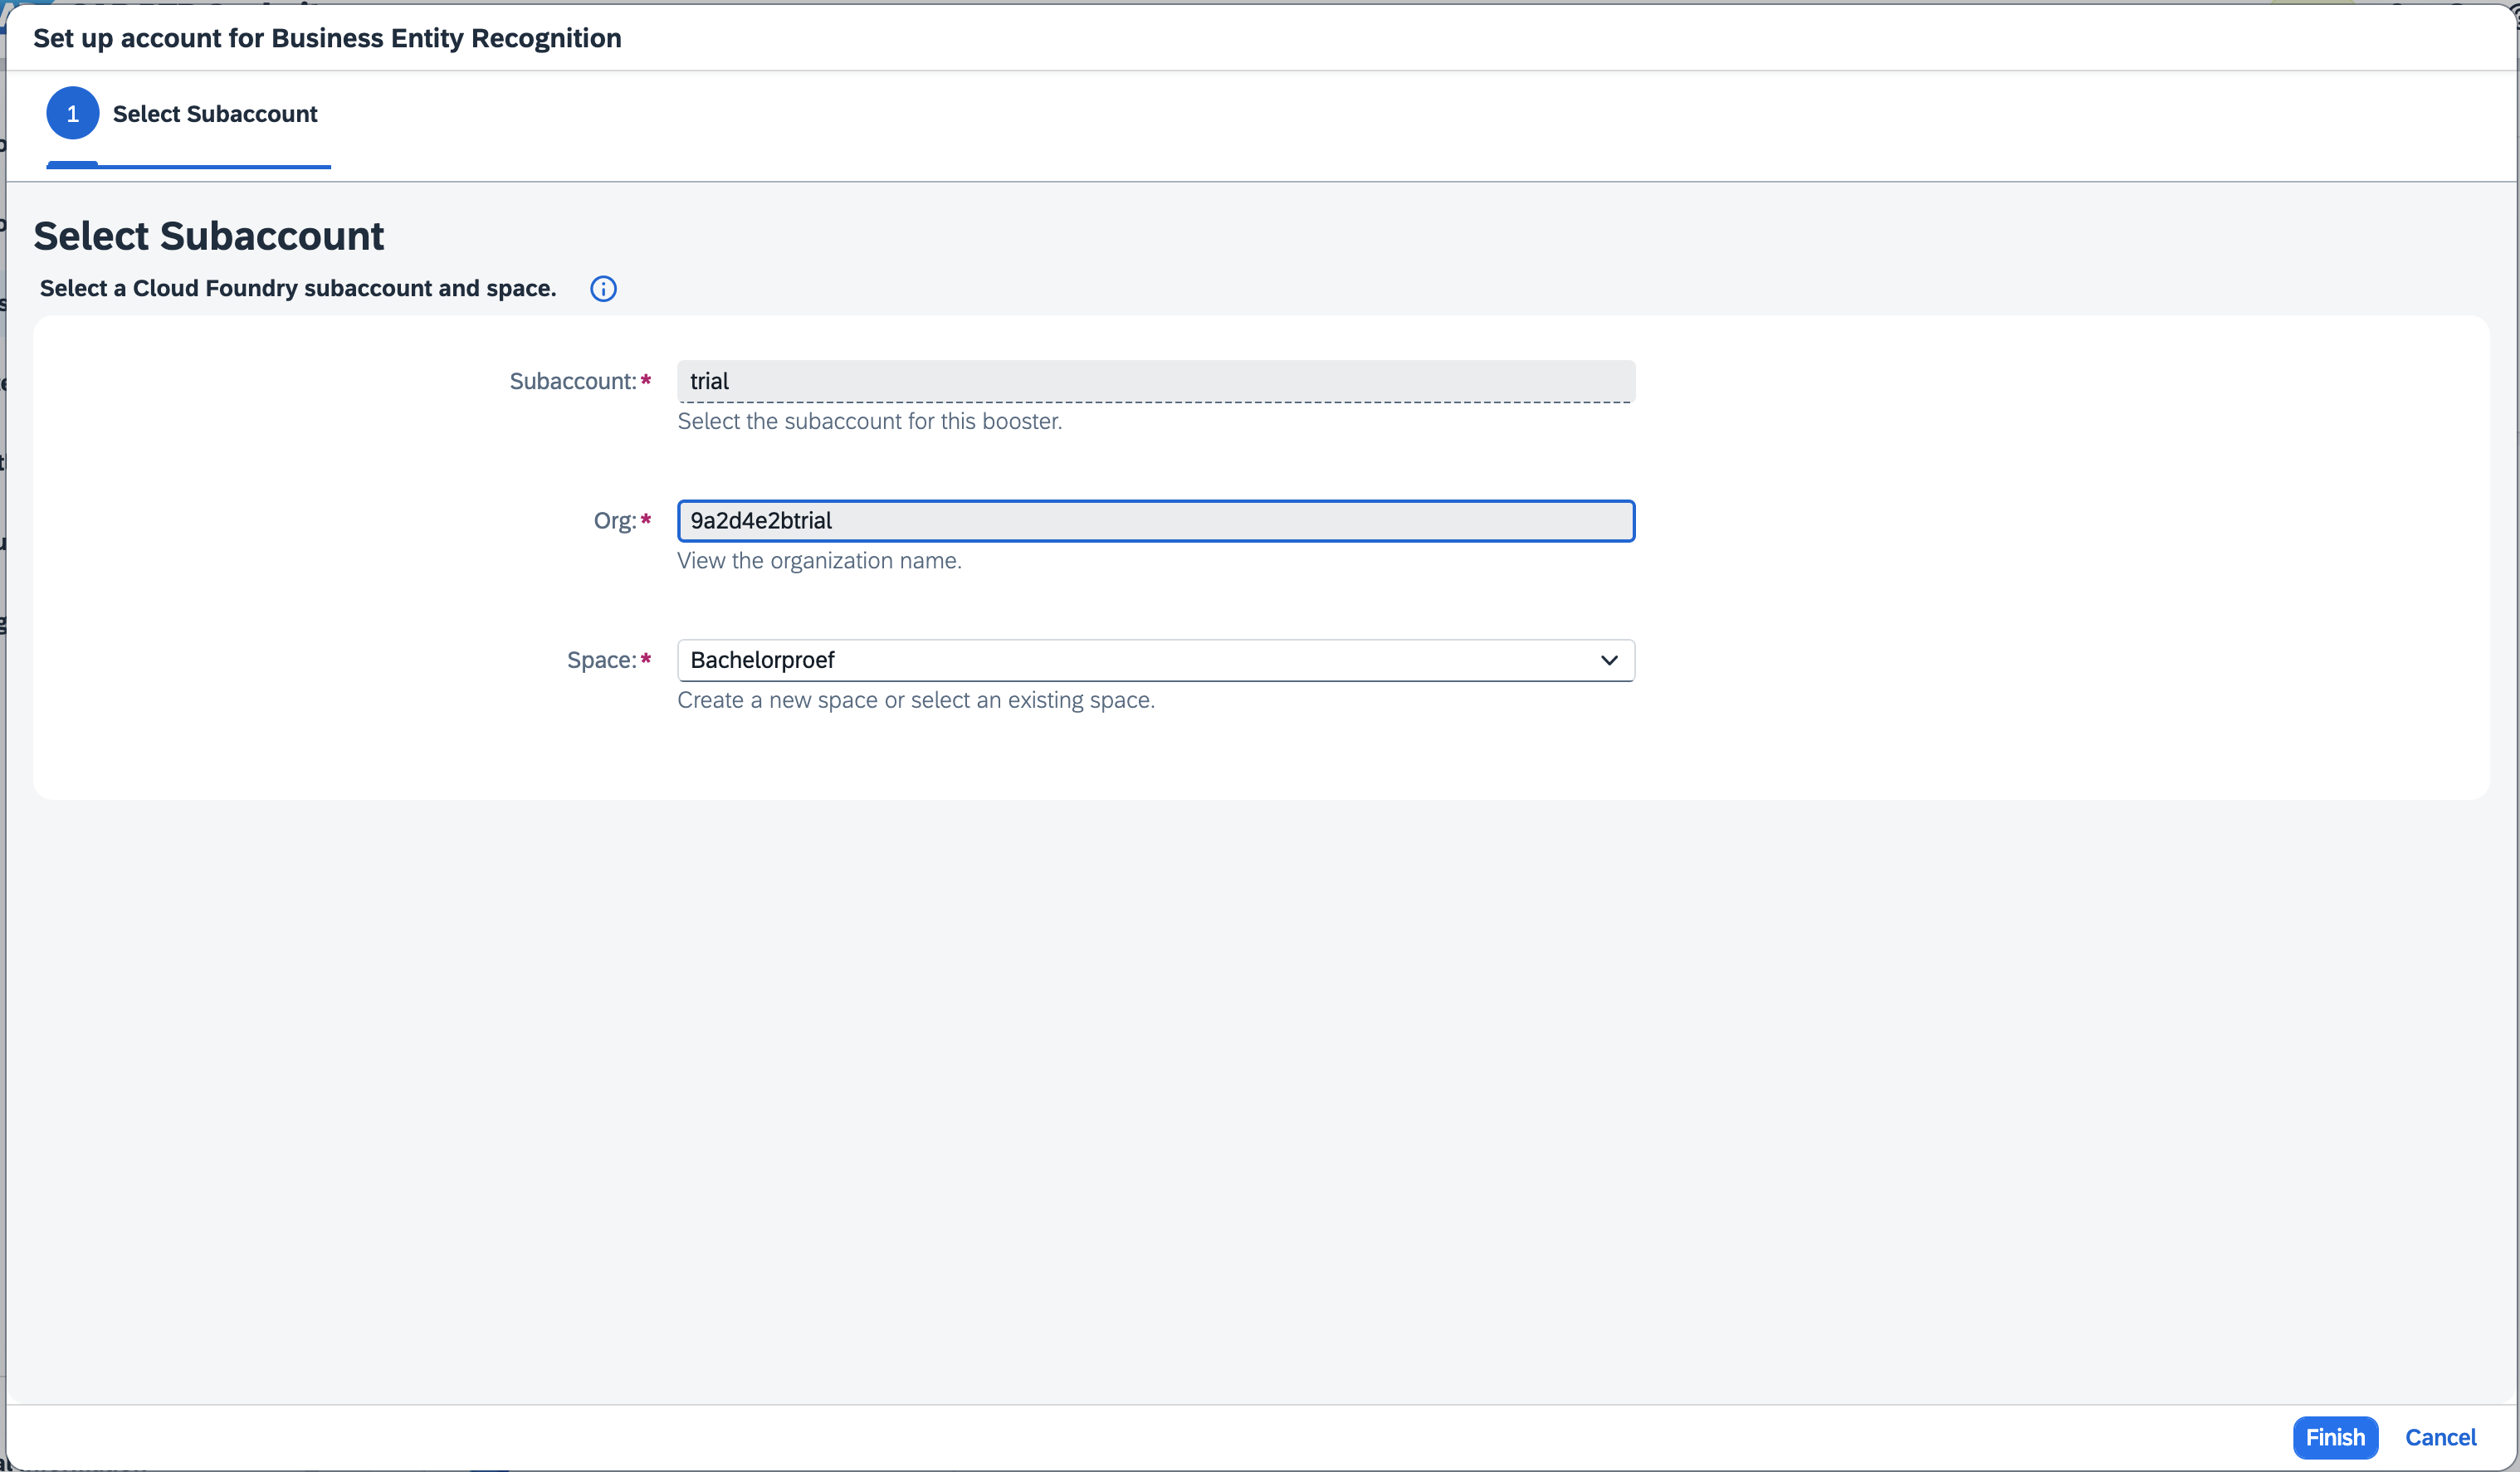
\includegraphics[width=0.8\textwidth]{./graphics/booster_subaccount.png}
    \caption{Booster subaccount selectie}
    \label{fig:booster-subaccount}
\end{figure}

\begin{figure}[H]
    \centering
    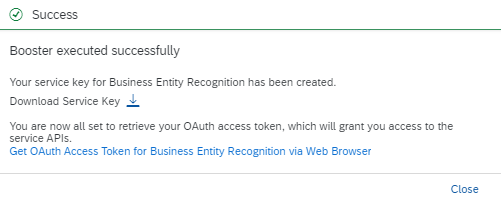
\includegraphics[width=0.8\textwidth]{./graphics/booster_succes.png}
    \caption{Booster succesvol uitgevoerd}
    \label{fig:booster-succes}
\end{figure}

\section{Python api}
\label{sec:python-api}

Om de Business Entity Recognition service te gebruiken heeft SAP een handige API beschikbaar gesteld die het mogelijk maakt om de service aan te roepen en te gebruiken. Hiervoor hebben ze ook een Python library gemaakt om dit gemakkelijk via code te gebruiken. Om een webapplicatie rond deze service te maken, zal er een eigen API gemaakt worden om zo meer controle te hebben over de data die er wordt opgevraagd en verstuurd.

Om de API in python te maken wordt er gebruik gemaakt van de Flask library. Flask is een library die het mogelijk maakt om snel verschillende soorten webapplicaties op te zetten. 

\subsection{Virtualenv en packages installeren}
Eerst wordt er doormiddel van virtualenv een nieuwe virtuele omgeving gemaakt. Er wordt een virtuele omgeving gemaakt omdat verschillende projecten verschillende dependencies kunnen hebben en deze op die manier niet met elkaar in conflict kunnen komen. Om een nieuwe virtuele omgeving te maken dient virtualenv geïnstalleerd met het volgende commando:
\begin{lstlisting}[language=bash]
    pip3 install virtualenv
\end{lstlisting}

Dan wordt er een map aangemaakt waarin de code zal komen, in dit voorbeeld wordt de map 'api' gemaakt waarin alle code van de api zal komen.
\begin{lstlisting}[language=bash]
    mkdir api
    cd api
\end{lstlisting}

Dan wordt de daadwerkelijke virtuele omgeving aangemaakt in de huidige map:

\begin{lstlisting}[language=bash]
    virtualenv .
\end{lstlisting}

Dit commando zorgt ervoor dat er virtuele omgeving in de map wordt gemaakt, het commando maakt ook een aantal mappen en bestanden aan die python nodig heeft om het project correct uit te voeren.
\begin{itemize}
    \item bin: Deze map bevat alle uitvoerbare bestanden die nodig zijn om de virtuele omgeving te activeren en te deactiveren.
    \item lib: Deze map bevat alle libraries die geïnstalleerd zijn in de virtuele omgeving.
    \item pyvenv.cfg: Dit bestand bevat de configuratie van de virtuele omgeving.
    \item .gitignore: Dit bestand bevat alle bestanden die niet mogen worden opgenomen in een git repository.
\end{itemize}

Uiteindelijk wordt de virtuele omgeving geactiveerd:
\begin{lstlisting}[language=bash]
    source bin/activate
\end{lstlisting}

Als de virtuele omgeving geactiveerd is, kan er begonnen worden met het installeren van de benodigde libraries. De libraries die geïnstalleerd moeten worden zijn de volgende:
\begin{itemize}
    \item Flask
    \item Flask-Cors
    \item sap-business-entity-recognition-client-library
\end{itemize}

Om deze libraries te installeren wordt er gebruik gemaakt van het volgende commando:
\begin{lstlisting}[language=bash]
    pip install Flask Flask-Cors sap-business-entity-recognition-client-library
\end{lstlisting}
Dit zal ervoor zorgen dat de libraries worden geïnstalleerd worden in de '/lib' map om later in de code te kunnen gebruiken.

Om de webserver te starten om de API te testen, wordt er gebruik gemaakt van het volgende commando:
\begin{lstlisting}[language=bash]
    flask run --reload
\end{lstlisting}

Dit commando zal de webserver starten en de API beschikbaar maken op \url{http://127.0.0.1:5000}. De optie '--reload' zorgt ervoor dat de webserver automatisch herstart wordt als er een aanpassing in de code wordt gemaakt. Dit maakt het gemakkelijker om de code te testen en aan te passen zonder dat de API constant manueel herstart moet worden.

\subsection{API code}

De code van de API wordt geplaatst in een bestand genaamd 'app.py'. De code bestaat uit een aantal methodes die de verschillende endpoints van de API vormen.
Om een API in flask te maken, worden eerst de verschillende dependencies geïmporteerd die in het project gebruikt zullen worden. Dan wordt er een instantie van de Flask klasse aangemaakt en wordt er een aantal configuraties ingesteld. De eerste endpoint die wordt aangemaakt is de '/health' endpoint. Deze endpoint is een eenvoudige methode die 'OK' antwoord om te controleren of de connectie met de API werkt.

\begin{listing}[H]
    \setminted{%
gobble=2,
}   
\begin{minted}{python3}
    from flask import Flask, jsonify, request
    from flask_cors import CORS, cross_origin
    from sap_ber_client import ber_api_client
    from time import sleep

    app = Flask(__name__)
    cors = CORS(app, origins="*")
    app.config['CORS_HEADERS'] = 'Content-Type'

    @app.route('/health')
    @cross_origin()
    def health():
        return jsonify("OK")
\end{minted}
\caption{Import van de dependencies en de '/health' endpoint in app.py}
\end{listing}

\paragraph{addAuth functie}
Om de Business Entity Recognition service te gebruiken wordt er een instantie van de ber\_api\_client klasse aangemaakt. Deze klasse heeft een aantal methodes die het mogelijk maken om de service te gebruiken. Om deze klasse te kunnen gebruiken, moet er eerst een aantal gegevens worden ingevuld die nodig zijn om de service te gebruiken. Hiervoor wordt er een methode 'addAuth' gebruikt die de gegevens van de gebruiker in elke vraag richting de API ophaalt en de instantie teruggeeft.
\begin{listing}[H]
    \setminted{%
gobble=2,
}   
\begin{minted}{python3}
    def addAuth(data):

    try:
        url = data['url']
        uaa_clientid = data['uaa']['clientid']
        uaa_clientsecret = data['uaa']['clientsecret']
        uaa_url = data['uaa']['url']
    
        return ber_api_client.BER_API_Client(url, uaa_clientid, 
                                    uaa_clientsecret, uaa_url)
    except:
        return None
\end{minted}
\caption{addAuth methode in app.py}
\end{listing}

\paragraph{API endpoints}

De api heeft een aantal endpoints die het mogelijk maken voor een gebruiker of applicatie om de service aan te roepen en een resultaat terug te krijgen. De '/models' route geeft een lijst van alle aanwezige modellen terug die gebruikt kunnen worden om een tekst te lezen. Op deze manier kan de gebruiker alle beschikbare modellen zien en kiezen welke hij wilt gebruiken. Deze modellen geven aan de BER-service wat context over wat voor tekst het precies is, wat betere resultaten op kan leveren.

De '/inference' route is de route die de tekst neemt samen met de naam van het model en die dit doorgeeft aan de BER-service. De service zal de tekst inlezen en de belanghebbende informatie eruit halen. De BER-service geeft een id terug van de 'job' die het document gekregen heeft, de methode wacht tot de service klaar is met het document te verwerken en haalt de informatie op aan de hand van dit id. De methode leest dan de resulaten in en geeft deze terug in een JSON formaat dat gemakkelijk te gebruiken is in de frontend applicatie.

\begin{listing}[H]
    \setminted{%
gobble=2,
}   
\begin{minted}{python3}
    @app.route('/models', methods=['POST'])
    @cross_origin()
    def getModels():
        ber_service = addAuth(request.get_json())

        if ber_service is None:
            return "No valid credentials provided", 400
    
        models = ber_service.get_trained_models()
        result = models.json()['data']['sapModels']['models']
        return jsonify({"items" : result})
\end{minted}
\caption{'/models' endpoint in app.py}
\end{listing}

\begin {listing}[H]
    \setminted{%
gobble=2,
}
\begin{minted}{python3}
    @app.route('/inference', methods=['POST'])
    @cross_origin()
    def inference():
        req_data = request.get_json()

        ber_service = addAuth(req_data['auth'])
        
        model_version = 1
        model_name = req_data['model']
        text = req_data['text']
        
        if ber_service is None:
            return "No valid credentials provided", 400
        

        inference_job = ber_service.post_inference_job(text,model_name, 
                                                        model_version)
        inference_jobid = inference_job.json()['data']['id']
        
        inference_job_result = ber_service.get_inference_job(inference_jobid)
        while inference_job_result.json()['data']['status'] == 'PENDING':
            inference_job_result = ber_service.get_inference_job(inference_jobid)
            sleep(1)

        response = inference_job_result.json()
        
        data = response['data']['result'][0]
        result = []
        for key in data.keys():
            if len(data[key]) == 0:
                merged = {"name": key, "value": '', "confidence": 0}
            else:
                merged = {"name": key} | data[key][0]
            result.append(merged)

        return jsonify({"items" : result})
\end{minted}
\caption{'/inference' endpoint in app.py}
\end{listing}

\paragraph{Note}
Om de code te laten werken, moet er een aanpassing gebeuren in de sap-business-entity-recognition-client-library. Deze gebruikt een verouderde versie van de requests library die ervoor zorgt dat de code niet werkt. Om dit op te lossen moet er in de \mintinline{bash}|/lib/sap_ber_client| map een aanpassing gebeuren aan de parameter in het \mintinline{bash}|http_request_retry.py| bestand. De parameter 'method\_whitelist' die wordt megegeven wordt aan het retry object moet worden aangepast naar 'allowed\_methods', zoals in codevoorbeeld \ref{code:allowed_methods}.
\begin{listing}[H]
    \setminted{
gobble=2,
}
\begin{minted}{python3}
    def retry_session(pool_maxsize=None, retries=3, backoff_factor=1,
    status_forcelist=(500, 502, 503, 504)):
    session = requests.Session()
    retry = Retry(total=retries,
                  read=retries,
                  status=retries,
                  connect=retries,
                  backoff_factor=backoff_factor,
                  status_forcelist=status_forcelist,
                  allowed_methods=['GET'],
                  raise_on_status=False)
    adapter = HTTPAdapter(max_retries=retry, pool_maxsize=pool_maxsize)
    session.mount('http://', adapter)
    session.mount('https://', adapter)
    return session
\end{minted}
\caption{Aanpassing in http\_request\_retry.py}
\label{code:allowed_methods}
\end{listing}

\section{Frontend applicatie}

In deze sectie wordt er toegelicht hoe de frontend applicatie is opgebouwd en hoe deze communiceert met de API die in sectie \ref{sec:python-api} is gemaakt. De frontend applicatie is een webapplicatie die gebruik maakt van SAP Fiori en is bedoeld om een gebruiksvriendelijke manier te bieden om de BER-service te gebruiken. 

\subsection{Opzetten van het Fiori project}

Om een Fiori-project aan te maken, biedt SAP een eenvoudige manier. In Visual Studio Code kan een nieuw project worden aangemaakt met behulp van de Fiori Application Generator. Deze generator biedt de mogelijkheid om een aantal zaken te configureren, zoals de naam, beschrijving en minimale versie van het project. Ook kan er een voorgebouwde template worden gekozen die een basis vormt voor het project en een externe data source zoals een SAP systeem. 

In deze proof of concept is er gekozen voor een basis template en zonder externe data source omdat deze later toegevoegd wordt in de code. De rest van de configuratie is de naam van de eerste view en het project zelf, zoals te zien is in figuur \ref{fig:fiori-generator}.

\begin{figure}[H]
    \centering
    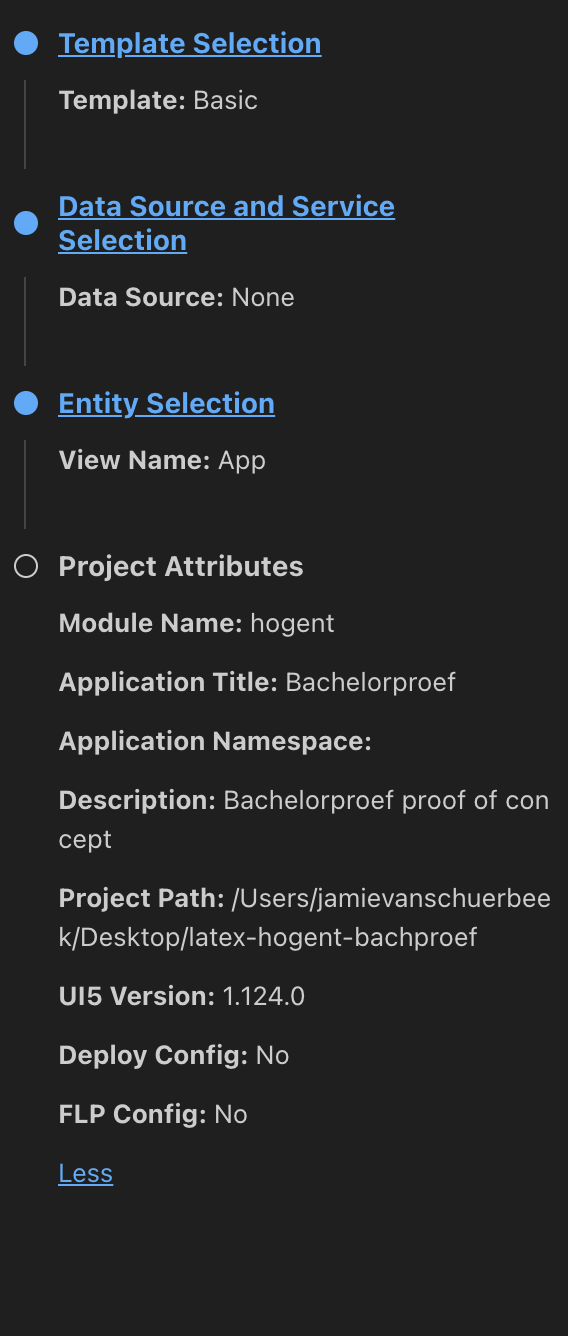
\includegraphics[scale=0.4]{./graphics/Fiori_config.png}
    \caption{Fiori application generator}
    \label{fig:fiori-generator}
\end{figure}

\subsection{Bestandenstructuur van de Fiori-applicatie}
De Fiori Application Generator maakt een aantal bestanden en mappen aan die het project correct laten werken. Deze structuur ziet er als volgt uit:

\begin{figure}[H]
    \centering
    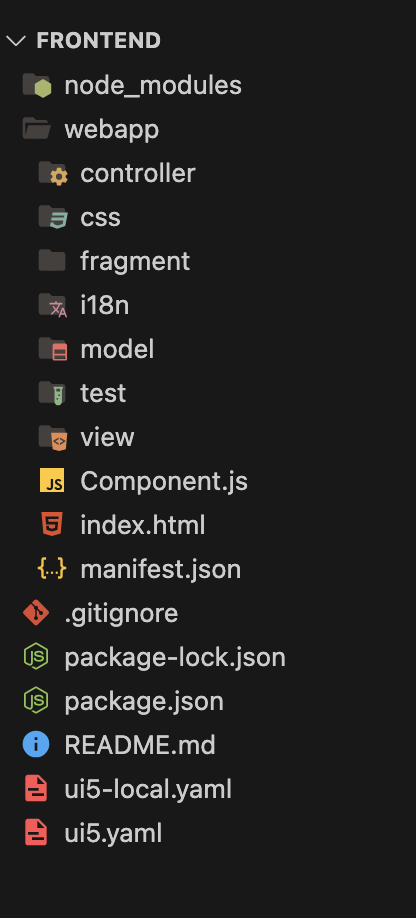
\includegraphics[scale=0.4]{./graphics/projectstructuur_fiori.png}
    \caption{Bestandenstructuur van het fiori project}
    \label{fig:fiori-generator}
\end{figure}

\begin{itemize}
    \item \textbf{node\_modules:} Bevat alle dependencies die aanwezig zijn in het project.
    \item \textbf{webapp:} Bevat alle code die de frontend van de applicatie vormt.
    \begin{itemize}
        \item \textbf{controller:} Bevat alle javascript controllers die de logica van de applicatie bedienen.
        \item \textbf{css:} Bevat alle css bestanden die de stijl van de app bepalen.
        \item \textbf{fragment: } Bevat alle fragments, dit zijn views die hergebruikt kunnen worden, zoals een dialoogvenster.
        \item \textbf{i18n:} Bevat alle vertalingen die de app ondersteunt.
        \item \textbf{model:} Bevat alle modellen die de app gebruikt, indien de app met een database zou werken.
        \item \textbf{test: } Bevat alle testen die geschreven zijn voor de app.
        \item \textbf{view:} Bevat alle views die de app heeft, deze views bepalen de structuur van de pagina.
        \item \textbf{Component.js:} Dit bestand is een component dat door ui5 wordt gemaakt die de app opstart.
        \item \textbf{index.html:} Dit bestand is de hoofdpagina van de app, hierin wordt de rest van de app in getoond.
        \item \textbf{manifest.json:} Dit bestand bevat alle configuratie van de app, zoals de naam, beschrijving en de versie.
    \end{itemize}
    \item \textbf{.gitignore:} Dit bestand bevat alle bestanden en mappen die niet mogen worden opgenomen in een git repository.
    \item \textbf{package.json en package-lock.json:} Deze bestanden bevatten alle info dependencies die nodig zijn om de app te laten werken.
    \item \textbf{ui5.yaml en ui5-local.yaml:} Deze bestanden bevatten alle ui5 configuratie.
\end{itemize}

\subsection{Eerste opstart}

Voordat de applicatie voor de eerste keer gestart kan worden, moeten eerst alle benodigde dependencies geïnstalleerd worden. Dit kan gedaan worden door het volgende commando uit te voeren.
\begin{lstlisting}[language=bash]
    npm install
\end{lstlisting}

Als dit commando uitgevoerd is, kan de applicatie voor het eerst gestart worden met het volgende commando:
\begin{lstlisting}[language=bash]
    npm start
\end{lstlisting}

Dit commando zal de ingebouwde webserver starten en de app openen in de webbrowser. 

\subsection{Code van de frontend: de views}

Als het project is opgezet, kan er begonnen worden met het effectief schrijven van de code die de frontend vormt. In dit onderzoek is er gekozen om alle functionaliteiten in één view te plaatsen. Dit zodat de gebruiker gemakkelijk alle functionaliteiten kan terugvinden en niet constant moet navigeren tussen verschillende paginas.

\paragraph{App view}

De app view is de eerst pagina die de gebruiker ziet als hij de app opent. In deze proof of concept is dit de enige pagina die de applicatie en deze heeft daarom heel veel elementen om alle functionaliteiten te kunnen gebruiken. 

Om een view te maken in SAP Fiori worden altijd een aantal namespaces gebruikt. Deze namespaces worden door SAP aangeboden om verschillende soorten voor gedefinieerde elementen te kunnen gebruiken voor verschillende doeleinden. In codevoorbeeld \ref{code:app-view} is te zien hoe de namespaces bovenaan de pagina worden geïmporteerd en hoe de basis van de pagina eruit ziet voor de rest van de componenten worden toegevoegd.

\begin{listing}[H]
    \setminted{%
gobble=2,
}
\begin{minted}{xml}
    <mvc:View controllerName="hogent.controller.App"
    xmlns:l="sap.ui.layout"
    xmlns:u="sap.ui.unified"
    xmlns:mvc="sap.ui.core.mvc" displayBlock="true"
    xmlns:core="sap.ui.core"
    xmlns:f="sap.f"
    xmlns:card="sap.f.cards"
    xmlns:tnt="sap.tnt"
    xmlns="sap.m">
    <Shell id="shell">
        <App id="app">
            <pages>
                <Page id="page" title="{i18n>title}">
                    <content>
                        <l:VerticalLayout>
                            <!-- REST VAN DE VIEW -->
                        </l:VerticalLayout>
                    </content>
                </Page>
            </pages>
        </App>
    </Shell>
</mvc:View>
\end{minted}
\caption{Namespaces importeren in app.view.xml}
\label{code:app-view}
\end{listing}

Als er een service key wordt geüpload, wordt er bovenaan de pagina een kaart getoond met alle gegevens van de huidige gebruiker. Ook wordt er een knop getoond die het mogelijk maakt om de huidige service key te veranderen indien een andere gebruiker de app wilt gebruiken. 
\begin{listing}[H]
    \setminted{%
gobble=2,
}
\begin{minted}{xml}
    <f:Card class="sapUiMediumMargin">
        <f:header>
            <card:Header title="User info"/>
        </f:header>
        <f:content>
            <VBox class="sapUiSmallMargin" justifyContent="SpaceBetween">
                <Text id="userClientId" text="Clientid: {auth>/uaa/clientid}"/>
                <Text id="userSubAccountId" text="Subaccountid: {auth>/uaa/subaccountid}"/>
                <Text id="userTennantId" text="Tennantid: {auth>/uaa/tenantid}"/>
                <HBox id="userApiHealth">
                    <Text text="API Health:"/>
                    <tnt:InfoLabel id="lblApiHealth" text="NOT AVAILABLE" colorScheme="2"/>
                </HBox>
                <Button text="change" press="openAuthDialog"/>
            </VBox>
        </f:content>
    </f:Card>
\end{minted}
\caption{User info kaart in app.view.xml}
\end{listing}

De belangrijkste functionaliteit van de app is het uploaden van een tekstbestand om daadwerkelijk een tekst te kunnen analyseren. Om dit te doen is er een fileuploader toegevoegd aan de pagina die het mogelijk maakt om een tekstbestand te kiezen op het apparaat van de gebruiker. Naast de fileuploader is er ook een menu toegevoegd die het mogelijk maakt om te kiezen uit een bestaand model om de context van de tekst te bepalen. De 'Upload file' knop zorgt dat in de controller het bestand naar de API wordt gestuurd zodat deze de tekst kan verwerken. Al deze zaken samen vormen de code die te zien is in codevoorbeeld \ref{code:fileuploader}.
\begin{listing}[H]
    \setminted{%
gobble=2,
}
\begin{minted}{xml}
    <u:FileUploader id="fileUploaderFS" name="fileUploaderFS" 
    uploadUrl="uploadFile" change="onFileChange" fileType="txt" 
    multiple="false" placeholder="Upload"/>
    <VBox alignContent="SpaceBetween">
        <Text text="Model"/>
        <ComboBox id="selectModel" items="{models>/items}">
            <core:Item key="{models>modelName}" text="{models>modelName}"/>
        </ComboBox>
    </VBox>
    <Button text="Upload File" press="handleUploadPress"/>
\end{minted}
\caption{Fileuploader en model selectie in app.view.xml}
\label{code:fileuploader}
\end{listing}

Als de API de tekst heeft verwerkt, wordt deze door de API teruggegeven in een JSON formaat. De controller zal deze data in een JSON model plaatsen zodat deze dat bereikbaar is in de view. De view zal dan de data in een tabel plaatsen zodat de gebruiker de resultaten kan zien.

\begin{listing}[H]
    \setminted{%
gobble=2,
}
\begin{minted}{xml}
    <Table headerText="Extracted entities" width="auto" 
    class="sapUiResponsiveMargin" items="{result>/items}">
            <columns>
                <Column>
                    <Text text="Name"/>
                </Column>
                <Column>
                    <Text text="Value"/>
                </Column>
                <Column>
                    <Text text="Confidence"/>
                </Column>
            </columns>
            <items>
                <ColumnListItem>
                    <cells>
                        <Text text="{result>name}"/>
                        <Text text="{result>value}"/>
                        <Text text="{result>confidence}"/>
                    </cells>
                </ColumnListItem>
            </items>
        </Table>
\end{minted}
\caption{Tabel met resultaten in app.view.xml}
\end{listing}

\paragraph{de UploadAuth fragment}
Om de service key toe te kunnen voegen, wordt er een dialoogvenster getoond die het mogelijk maakt om de service key te uploaden. Voor dit dialoogvenster wordt er een fragment view gemaakt waarin de structuur van het venster wordt bepaald.

Het dialoogvenster wordt getoond als de gebruiker de applicatie opent of als de gebruiker op de 'change' knop drukt. Als de gebruiker de service key heeft toegevoegd, wordt deze in de controller opgeslagen zodat deze kan worden gebruikt elke keer als de API wordt aangeroepen.

Bij het dialog-element wordt het \mintinline{xml}|afterClose| attribuut gebruikt om een methode aan te roepen in de controller als het dialoogvenster wordt gesloten. Dit zorgt ervoor dat de service key wordt opgeslagen in de controller en dat deze kan worden gebruikt in de rest van de applicatie.

\begin{listing}[H]
    \setminted{%
gobble=2,
}
\begin{minted}{xml}
    <core:FragmentDefinition xmlns="sap.m"
    xmlns:core="sap.ui.core"
    xmlns:l="sap.ui.layout"
    xmlns:u="sap.ui.unified"
    xmlns:f="sap.ui.layout.form">
    <Dialog id="dlgUploadAuth" title="Please upload your key.json" 
    afterClose="onAuthClose">
        <u:FileUploader id="authUploader" name="authUploader" 
        uploadUrl="uploadFile" change="onAuthFileChanged" multiple="false" 
        placeholder="Upload key.json" 
        typeMissmatch="typeMissmatch" fileSizeExceed="fileSizeExceed" />
    </Dialog>
</core:FragmentDefinition>
\end{minted}
\end{listing}

\subsection{Code van de frontend: de controller}

De controller zorgt ervoor dat er logica aan de view wordt toegevoegd. In de controller worden verschillende methodes gemaakt die uitgevoerd worden na een bepaalde actie in de view. 

\paragraph{De onInit en openAuthDialog methodes}

Een controller in een Fiori project begint eerst met het importeren van alle benodigde dependencies, deze worden als parameter doorgegeven aan de controller om ze daar te gebruiken. In de controller is er altijd eerst de \mintinline{javascript}|onInit| methode aanwezig die wordt aangeroepen als de pagina wordt geopende. In dit geval wordt hier de functie aangeroepen die het dialoogvenster opent om de service key te uploaden.

De \mintinline{javascript}|openAuthDialog| functie in de controller zorgt ervoor er geen bestaande dialoogvenster geopend is en daarna dat de fragment wordt ingeladen en getoond aan de gebruiker. 

De \mintinline{javascript}|onAuthClose| functie wordt uitgevoerd als het dialoogvenster wordt gesloten. Deze functie zorgt ervoor dat het venster correct wordt gesloten en dat de rest van de data in de applicatie wordt opgehaald.

\begin{listing}[H]
    \setminted{%
gobble=2,
}
\begin{minted}{javascript}
    sap.ui.define(
    [
        "sap/ui/core/mvc/Controller",
        "sap/ui/model/json/JSONModel",
        "sap/m/MessageToast",
    ],
    /**
     * @param {typeof sap.ui.core.mvc.Controller} Controller
     */
    function (Controller, JSONModel, MessageToast) {
        "use strict";

        const url = "http://127.0.0.1:5000";

        return Controller.extend("hogent.controller.App", {
        onInit: function () {
            this.openAuthDialog();
        },
        
        // REST VAN DE METHODES

        //Open auth dialog
        openAuthDialog: function () {
            if (this.byId("dlgUploadAuth")) {
                this.byId("dlgLogin").destroy();
                this.pDialog = null;
            }
            this.pDialog = this.loadFragment({
                name: "hogent.fragment.UploadAuth",
            });
            this.pDialog.then(function (oDialog) {
                oDialog.open();
            });
        },

            onAuthClose: function () {
            this.byId("dlgUploadAuth").destroy();
            this.pDialog = null;

            this.addUserInfo();
            this.fetchModels();
            },
        });
    });
\end{minted}
\caption{onInit en openAuthDialog methodes in App.controller.js}
\end{listing}


\paragraph{De addUserInfo en fetchModels methode}

De \mintinline{javascript}|addUserInfo| methode is een simple methode die de API aanroept en wacht op een antwoord. Als de API een antwoord teruggeeft wordt dit in de view geplaatst zodat de gebruiker kan zien dat de connectie met de API in orde is.

De \mintinline{javascript}|fetchModels| methode is een methode die de API aanroept om alle beschikbare modellen op te halen. Deze modellen worden dan in een JSON model geplaatst zodat deze in de view beschikbaar zijn om aan de gebruiker te laten zien.

\begin{listing}[H]
    \setminted{%
gobble=2,
}
\begin{minted}{javascript}
    //get all available models
    fetchModels: function () {
        fetch(url + "/models", {
          method: "POST",
          headers: {
            "Content-Type": "application/json",
          },
          body: JSON.stringify(this.getView().getModel("auth").getData()),
        })
          .then((response) => {
            return response.json();
          })
          .then((data) => {
            this.getView().setModel(new JSONModel(data), "models");
          });
      },

      //check if connection to API is OK
    addUserInfo: function () {
        var pUrl = url + "/health";

        fetch(pUrl, {
          method: "GET",
        })
          .then((response) => {
            return response.json();
          })
          .then((data) => {
            this.getView()
              .byId("lblApiHealth")
              .setText(data)
              .setColorScheme(data === "OK" ? 8 : 2);
          });
      },
\end{minted}
\caption{addUserInfo en fetchModels methodes in App.controller.js}
\end{listing}

\paragraph{De onFileChange methodes}

De \mintinline{javascript}|onFileChange| en \mintinline{javascript}|onAuhtFileChange| methodes zijn twee gelijkaardige methodes die worden aangeroepen als de gebruiker een bestand heeft gekozen in de fileuploader. Deze methodes zorgen ervoor dat het bestand in de controller via een JSON model wordt opgeslagen zodat deze kunnen gebruikt worden bij het verder oproepen van de API. Zij zullen zorgen dat wanneer de service key is geüpload, deze in de oproepen naar de API kunnen worden meegestuurd en dat het tekstbestand kan worden geüpload naar de API. 

\begin{listing}[H]
    \setminted{%
gobble=2,
}
\begin{minted}{javascript}
    //Hadle file change - read file content and store locally
    onFileChange: function (e) {
        var file = e.getParameter("files") && e.getParameter("files")[0];
        if (file && window.FileReader) {
          var reader = new FileReader();
          reader.onload = function (evn) {
            var strCSV = evn.target.result;
            console.log(strCSV);
            this.getView().setModel(
              new JSONModel({ text: strCSV }),
              "currentText"
            );
          }.bind(this);
          reader.readAsText(file);
        }
      },

      //Handle file change - change file on api
      onAuthFileChanged: function (e) {
        var file = e.getParameter("files") && e.getParameter("files")[0];
        if (file && window.FileReader) {
          var reader = new FileReader();
          reader.onload = function (evn) {
            var strCSV = evn.target.result;
            this.getView().setModel(new JSONModel(JSON.parse(strCSV)), "auth");

            this.byId("dlgUploadAuth").close();
          }.bind(this);
          reader.readAsText(file);
        }
      },
\end{minted}
\caption{onFileChange en onAuthFileChange methodes in App.controller.js}
\end{listing}

\paragraph{De handleUploadPress methode}

Één van de belangrijkste methodes in de controller is de \mintinline{javascript}|handleUploadPress| methode. Deze methode zorgt ervoor dat de tekst die de gebruiker wilt analyseren wordt geüpload naar de API. Deze methode wacht dan op het antwoord van de API en slaat deze op in de controller, zodat deze in de view in een overzichtelijke tabel kan worden getoond aan de gebruiker. 

\begin{listing}[H]
    \setminted{%
gobble=2,
}
\begin{minted}{javascript}
    handleUploadPress: function () {
        var pModel = this.getView().byId("selectModel").getSelectedItem();
        if (pModel === null) {
          MessageToast.show("No model selected");
          return;
        }

        fetch(url + "/inference", {
          method: "POST",
          headers: {
            "Content-Type": "application/json",
          },
          body: JSON.stringify({
            model: pModel.getKey(),
            auth: this.getView().getModel("auth").getData(),
            text: this.getView().getModel("currentText").getData().text,
          }),
        })
          .then((response) => {
            return response.json();
          })
          .then((data) => {
            console.log(data);
            this.getView().setModel(new JSONModel(data), "result");
          });
      }, 
\end{minted}
\caption{handleUploadPress methode in App.controller.js}
\end{listing}


%\input{...}
%\input{...}
%...

%%=============================================================================
%% Conclusie
%%=============================================================================

\chapter{Conclusie}%
\label{ch:conclusie}

% TODO: Trek een duidelijke conclusie, in de vorm van een antwoord op de
% onderzoeksvra(a)g(en). Wat was jouw bijdrage aan het onderzoeksdomein en
% hoe biedt dit meerwaarde aan het vakgebied/doelgroep? 
% Reflecteer kritisch over het resultaat. In Engelse teksten wordt deze sectie
% ``Discussion'' genoemd. Had je deze uitkomst verwacht? Zijn er zaken die nog
% niet duidelijk zijn?
% Heeft het onderzoek geleid tot nieuwe vragen die uitnodigen tot verder 
%onderzoek?

Na het uitvoeren van dit onderzoek kan er geconcludeerd worden dat het zeker mogelijk is om met machine learning technologie bedrijfsdocument te analyseren en hieruit relevante masterdata te halen. Om een antwoord te geven op de onderzoeksvraag "Hoe kan machine learning-technologie worden toegepast om relevante masterdata uit bedrijfsdocumenten te halen?" is de proof of concept een voorbeeld van hoe dit gebruikt kan worden, doormiddel van de SAP Business Entity Recognition service.

Het antwoord op de deelvraag 'welke tools bestaan er om dergelijke oplossingen te maken' is terug te vinden in de literatuurstudie in sectie \ref{sec:libraries}. Hieruit is gebleken dat er verschillende tools worden aangeboden, zowel open-source als betalende tools, die als oplossing kunnen dienen om dergelijke applicaties te maken. 

Tijdens het maken van de proof of concept is gebleken dat de BER service van SAP een tool is die verassend gemakkelijk te gebruiken is en die erg goede resultaten geeft. Doordat de BER service weinig configuratie nodig heeft, maakt het een ideale tool om snel een soortgelijke applicatie te maken. Het grootste nadeel van deze tool is dat het niet gratis is wat het minder aantrekkelijk maakt voor kleinere bedrijven.

De proof of concept maken met SAP Fiori was ook een aangename manier om een applicatie te maken. De tools en documentatie die SAP aanbied zijn erg uitgebreid en maken het op die manier erg gemakkelijk om een applicatie te maken. Dit maakt het dan ook in de toekomst mogelijk om de proof of concept verder uit te breiden en te integreren in een bestaande SAP omgeving.

%---------- Bijlagen -----------------------------------------------------------

\appendix

\chapter{Onderzoeksvoorstel}

Het onderwerp van deze bachelorproef is gebaseerd op een onderzoeksvoorstel dat vooraf werd beoordeeld door de promotor. Dat voorstel is opgenomen in deze bijlage.

%% TODO: 
%\section*{Samenvatting}

% Kopieer en plak hier de samenvatting (abstract) van je onderzoeksvoorstel.

% Verwijzing naar het bestand met de inhoud van het onderzoeksvoorstel
%---------- Inleiding ---------------------------------------------------------

\section{Introductie}%
\label{sec:introductie}

%Waarover zal je bachelorproef gaan? Introduceer het thema en zorg dat volgende zaken zeker duidelijk aanwezig zijn:
%
%\begin{itemize}
%  \item kaderen thema
%  \item de doelgroep
%  \item de probleemstelling en (centrale) onderzoeksvraag
%  \item de onderzoeksdoelstelling
%\end{itemize}
%
%Denk er aan: een typische bachelorproef is \textit{toegepast onderzoek}, wat betekent dat je start vanuit een concrete probleemsituatie in bedrijfscontext, een \textbf{casus}. Het is belangrijk om je onderwerp goed af te bakenen: je gaat voor die \textit{ene specifieke probleemsituatie} op zoek naar een goede oplossing, op basis van de huidige kennis in het vakgebied.
%
%De doelgroep moet ook concreet en duidelijk zijn, dus geen algemene of vaag gedefinieerde groepen zoals \emph{bedrijven}, \emph{developers}, \emph{Vlamingen}, enz. Je richt je in elk geval op it-professionals, een bachelorproef is geen populariserende tekst. Eén specifiek bedrijf (die te maken hebben met een concrete probleemsituatie) is dus beter dan \emph{bedrijven} in het algemeen.
%
%Formuleer duidelijk de onderzoeksvraag! De begeleiders lezen nog steeds te veel voorstellen waarin we geen onderzoeksvraag terugvinden.
%
%Schrijf ook iets over de doelstelling. Wat zie je als het concrete eindresultaat van je onderzoek, naast de uitgeschreven scriptie? Is het een proof-of-concept, een rapport met aanbevelingen, \ldots Met welk eindresultaat kan je je bachelorproef als een succes beschouwen?

In deze tijd is data niet meer weg te denken en is het een van de belangrijkste zaken in de bedrijfswereld, een bedrijf dat dan ook efficiënt omgaat met zijn master data kan op die manier meer geïnformeerde beslissingen maken. Omdat het ophalen van interessante data uit bedrijfsdocumenten voor veel bedrijven nog een manuele taak blijft, is een oplossing die meer geautomatiseerd is steeds interessanter aan het worden.  De bedoeling van dit onderzoek is manieren te vinden om relevante informatie uit bedrijfsdocumenten te halen, nadien een werkend prototype te maken voor deze oplossing en dit te integreren in het SAP Master Data Governance platform om op deze manier master data records aan te maken. Op deze manier kan met behulp van machine learning de anderzijds manuele taak van informatie extractie geautomatiseerd worden.

%---------- Stand van zaken ---------------------------------------------------

\section{State-of-the-art}%
\label{sec:state-of-the-art}

%Hier beschrijf je de \emph{state-of-the-art} rondom je gekozen onderzoeksdomein, d.w.z.\ een inleidende, doorlopende tekst over het onderzoeksdomein van je bachelorproef. Je steunt daarbij heel sterk op de professionele \emph{vakliteratuur}, en niet zozeer op populariserende teksten voor een breed publiek. Wat is de huidige stand van zaken in dit domein, en wat zijn nog eventuele open vragen (die misschien de aanleiding waren tot je onderzoeksvraag!)?
%
%Je mag de titel van deze sectie ook aanpassen (literatuurstudie, stand van zaken, enz.). Zijn er al gelijkaardige onderzoeken gevoerd? Wat concluderen ze? Wat is het verschil met jouw onderzoek?
%
%Verwijs bij elke introductie van een term of bewering over het domein naar de vakliteratuur, bijvoorbeeld~\autocite{Hykes2013}! Denk zeker goed na welke werken je refereert en waarom.
%
%Draag zorg voor correcte literatuurverwijzingen! Een bronvermelding hoort thuis \emph{binnen} de zin waar je je op die bron baseert, dus niet er buiten! Maak meteen een verwijzing als je gebruik maakt van een bron. Doe dit dus \emph{niet} aan het einde van een lange paragraaf. Baseer nooit teveel aansluitende tekst op eenzelfde bron.
%
%Als je informatie over bronnen verzamelt in JabRef, zorg er dan voor dat alle nodige info aanwezig is om de bron terug te vinden (zoals uitvoerig besproken in de lessen Research Methods).
%
%% Voor literatuurverwijzingen zijn er twee belangrijke commando's:
%% \autocite{KEY} => (Auteur, jaartal) Gebruik dit als de naam van de auteur
%%   geen onderdeel is van de zin.
%% \textcite{KEY} => Auteur (jaartal)  Gebruik dit als de auteursnaam wel een
%%   functie heeft in de zin (bv. ``Uit onderzoek door Doll & Hill (1954) bleek
%%   ...'')
%
%Je mag deze sectie nog verder onderverdelen in subsecties als dit de structuur van de tekst kan verduidelijken.

Information Extraction(IE) is een manier om tekst te doorzoeken met als doel relevante informatie voor de belanghebbende te vinden. Het omvangt meer dan enkel en alleen trefwoorden te zoeken in de tekst, maar de doelstellingen blijven achter bij het probleem van tekstbegrip, waarbij we proberen alle informatie in een tekst vast te leggen, samen met de intentie van de schrijver \autocite{hobbs2010}. Vroegere IE systemen waren meer gelimiteerd en konden namen, relaties en gebeurtenissen uit simpele teksten halen die een vaste structuur hadden, zoals ``locatie werd gebombardeerd'' en ``persoon werd aangenomen''. De nieuwste systemen van tegenwoordig kunnen door machine learning veel meer zaken herkennen waaronder meer domeinspecifieke zaken zoals ziekten, wetten en wetenschappelijke resultaten \autocite{Small2014}.

IE ligt tussen twee andere methodes van tekstverwerking, namelijk information retrieval en natuurlijke taalverwerking. IE kan worden beschouwd als een soort goedkoop, gericht begrijpen van natuurlijke taal. IE gaat uit van een verzameling documenten, waarin elk document namen en gebeurtenissen beschrijft die op elkaar lijken, maar waar de details verschillen. Voor een IE-taak wordt er een sjabloon voorzien die beschrijft wat voor informatie er in het document staat \autocite{Freitag2000}

Document information extraction(DOX) is een dienst aangeboden door SAP die het mogelijk maakt om met machine learning informatie uit documenten te halen. Op deze manier wordt het verwerken van grote hoeveelheden aan documenten die hun inhoud in titels en tabellen hebben verwerkt. Dit geeft de mogelijkheid om documenten zoals facturen en betalingsdocumenten automatisch te verwerken \autocite{SAPDOX}.

Business entity recognition(BER) is een gelijkaardige dienst die wordt aangeboden door SAP. Het grootste verschil is dat BER het mogelijk maakt om informatie uit ongestructureerde stukken tekst te halen. Dit biedt de mogelijkheid om bijvoorbeeld de context uit e-mails te halen of het automatiseren van herhalende taken zoals het beantwoorden van vragen over de status en betaling van facturen. Hier kun je voorgetrainde modellen gebruiken of eigen modellen om ervoor te zorgen dat de resultaten geschikter zijn voor de doeleinden van de gebruiker. Deze toepassing kan helpen om het manuele en herhalende werk in een bedrijf te verminderen zodat werknemers meer tijd hebben om zich te focussen op belangrijkere zaken.
 \autocite{SAPBER}
%---------- Methodologie ------------------------------------------------------
\section{Methodologie}%
\label{sec:methodologie}

%Hier beschrijf je hoe je van plan bent het onderzoek te voeren. Welke onderzoekstechniek ga je toepassen om elk van je onderzoeksvragen te beantwoorden? Gebruik je hiervoor literatuurstudie, interviews met belanghebbenden (bv.~voor requirements-analyse), experimenten, simulaties, vergelijkende studie, risico-analyse, PoC, \ldots?
%
%Valt je onderwerp onder één van de typische soorten bachelorproeven die besproken zijn in de lessen Research Methods (bv.\ vergelijkende studie of risico-analyse)? Zorg er dan ook voor dat we duidelijk de verschillende stappen terug vinden die we verwachten in dit soort onderzoek!
%
%Vermijd onderzoekstechnieken die geen objectieve, meetbare resultaten kunnen opleveren. Enquêtes, bijvoorbeeld, zijn voor een bachelorproef informatica meestal \textbf{niet geschikt}. De antwoorden zijn eerder meningen dan feiten en in de praktijk blijkt het ook bijzonder moeilijk om voldoende respondenten te vinden. Studenten die een enquête willen voeren, hebben meestal ook geen goede definitie van de populatie, waardoor ook niet kan aangetoond worden dat eventuele resultaten representatief zijn.
%
%Uit dit onderdeel moet duidelijk naar voor komen dat je bachelorproef ook technisch voldoen\-de diepgang zal bevatten. Het zou niet kloppen als een bachelorproef informatica ook door bv.\ een student marketing zou kunnen uitgevoerd worden.
%
%Je beschrijft ook al welke tools (hardware, software, diensten, \ldots) je denkt hiervoor te gebruiken of te ontwikkelen.
%
%Probeer ook een tijdschatting te maken. Hoe lang zal je met elke fase van je onderzoek bezig zijn en wat zijn de concrete \emph{deliverables} in elke fase?

Het onderzoek zal voornamelijk uit 3 grote delen bestaan.
Het eerste deel zal een grote analyse zijn van een tweetal weken, met als doel goede kennis te krijgen over het onderwerp. Dit zal bestaan uit een studie van de verschillende methodes om informatie uit documenten te halen. Hier wordt algemene kennis over de verschillende methodes opgedaan over wat ze precies zijn en hoe ze werken. Later zal dit toegepast worden op de diensten en hulpmiddelen die ter beschikking worden gesteld om dergelijke toepassingen te maken. Er wordt dan een uitgebreide studie gedaan van de documentatie en artikelen van professionals in het vakgebied. Er wordt tijdens deze studie naar een aantal verschillende parameters gekeken, namelijk: prijs, gebruiksgemak, kwaliteit en de mogelijkheid tot integratie met SAP platformen.

Als het eerste deel afgerond is zal er in het volgende deel eerst een aantal experimenten volgen om de theorie van het eerste deel te kunnen testen in de praktijk. In deze fase wordt vooral naar gebruiksgemak en kwaliteit gekeken. Er zal een aantal testen opgezet worden die verschillende diensten uitproberen, om zo te kunnen kijken met welke service gemakkelijk een document extractie-service kan gebouwd worden die kwalitatieve master data levert. Uit de resultaten van deze testen zal een service gekozen worden waarmee een concrete toepassing gebouwd kan worden in de vorm van een proof of concept(PoC). 

In het laatste deel van dit onderzoek is het hoofdzakelijk de bedoeling om de PoC te implementeren in het SAP master data governance platform. Op deze manier kan de master data die uit documenten gehaald wordt direct in SAP gebruikt worden. Nadien zal de toepassing uitermate getest en gebenchmarked worden om de verschillende prestaties van de toepassing te krijgen zoals snelheid en kwaliteit van de data. Op deze manier kan er een uitgebreide conclusie te kunnen maken met een antwoord op de onderzoeksvraag en prestaties van de toepassing.

%---------- Verwachte resultaten ----------------------------------------------
\section{Verwacht resultaat, conclusie}%
\label{sec:verwachte_resultaten}

%Hier beschrijf je welke resultaten je verwacht. Als je metingen en simulaties uitvoert, kan je hier al mock-ups maken van de grafieken samen met de verwachte conclusies. Benoem zeker al je assen en de onderdelen van de grafiek die je gaat gebruiken. Dit zorgt ervoor dat je concreet weet welk soort data je moet verzamelen en hoe je die moet meten.
%
%Wat heeft de doelgroep van je onderzoek aan het resultaat? Op welke manier zorgt jouw bachelorproef voor een meerwaarde?
%
%Hier beschrijf je wat je verwacht uit je onderzoek, met de motivatie waarom. Het is \textbf{niet} erg indien uit je onderzoek andere resultaten en conclusies vloeien dan dat je hier beschrijft: het is dan juist interessant om te onderzoeken waarom jouw hypothesen niet overeenkomen met de resultaten.

Het verwachte resultaat op het einde van het onderzoek is een antwoord op de onderzoeksvraag doormiddel van een werkend proof of concept van een applicatie die gebruikt kan worden voor verschillende doeleinden in een SAP-systeem. Deze proof of concept zou documenten als input moeten kunnen krijgen en de applicatie zou correcte info moeten teruggeven met betrekking tot de toepassing waar het gebruikt wordt. Er zijn verschillende tools en diensten beschikbaar om het ontwikkelen van zulke applicaties mogelijk en zelfs gemakkelijker te maken. De snelheid waarop het ophalen van info gebeurt is in dit onderzoek minder van belang, vooral de correctheid en relevantie van de data is de grootste prioriteit die gelegd wordt.


%%---------- Andere bijlagen --------------------------------------------------
% TODO: Voeg hier eventuele andere bijlagen toe. Bv. als je deze BP voor de
% tweede keer indient, een overzicht van de verbeteringen t.o.v. het origineel.
%\input{...}

%%---------- Backmatter, referentielijst ---------------------------------------

\backmatter{}

\setlength\bibitemsep{2pt} %% Add Some space between the bibliograpy entries
\printbibliography[heading=bibintoc]
\end{document}
